\documentclass[a4paper,12pt]{report}

\usepackage[brazilian,english]{babel}
\usepackage{indentfirst}
\usepackage{a4wide}
\usepackage[section]{placeins}
\usepackage[utf8]{inputenc}
% \usepackage[Conny]{fncychap}
\usepackage[T1]{fontenc}
\usepackage{txfonts}
\usepackage{type1cm}
\usepackage{courier}
\usepackage[scaled]{helvet}
\usepackage{epigraph}
\renewcommand*\familydefault{\sfdefault}

\hyphenation{
  es-ta-be-le-ci-do
  a-de-qua-da-men-te
  pro-ble-mas
  di-men-sio-na-men-to
  mo-de-lo
}

% Controlar linhas orfas e viuvas
\clubpenalty=10000
\widowpenalty=10000
\displaywidowpenalty=10000

% Formatar notas de rodape
\usepackage[hang]{footmisc}
\setlength{\footnotemargin}{1em}

\usepackage{url}
%% Define a new 'leo' style for the package that will use a smaller font.
\makeatletter
\def\url@leostyle{%
  \@ifundefined{selectfont}{\def\UrlFont{\sf}}{\def\UrlFont{\small\ttfamily}}}
\makeatother
%% Now actually use the newly defined style.
\urlstyle{leo}

\usepackage[left=3cm,top=3cm,right=2cm,bottom=2cm,includehead,ignoremp]{geometry}

\usepackage[small]{titlesec}
% \titlespacing{\chapter}{0pt}{-50pt}{*20}[0pt]
\titlespacing{\chapter}{0pt}{*-10}{*5}

% Running Headers and footers
\usepackage{fancyhdr}
% \pagestyle{fancy}
\pagestyle{headings}
% Redefine plain page style
\fancypagestyle{plain}{
  \fancyhf{}
  \renewcommand{\headrulewidth}{0pt}
  \fancyhead[LE,RO]{\thepage}
}

\linespread{1.3}
%\pdfpagewidth=\paperwidth
%\pdfpageheight=\paperheight

% Para habilitar cálculos em dimensões
\usepackage{calc}

% Multipart figures
%\usepackage{subfigure}

% More symbols
%\usepackage{amsmath}
%\usepackage{amssymb}
%\usepackage{latexsym}

% Surround parts of graphics with box
\usepackage{boxedminipage}

% Package for including code in the document
\usepackage{listings}

% If you want to generate a toc for each chapter (use with book)
%\usepackage{minitoc}

% This is now the recommended way for checking for PDFLaTeX:
\usepackage{ifpdf}

\ifpdf
\usepackage[pdftex]{graphicx}
\else
\usepackage{graphicx}
\fi

\title{Dionisio}
\author{Allan Douglas R. de Oliveira \\ allandouglas@gmail.com \and
Leonardo Nicacio Bessa \\ leobessa@gmail.com \and
Thiago Rodrigues Andrade \\ suffragium@gmail.com}
\date{2009-12-07}

\usepackage[absolute]{textpos}
\begin{document}

\ifpdf
\DeclareGraphicsExtensions{.png, .pdf, .jpg, .tif}
\else
\DeclareGraphicsExtensions{.eps, .jpg}
\fi

%\maketitle
\pagestyle{empty}
\begin{center}
  {\large ALLAN DOUGLAS R. DE OLIVEIRA \\
    LEONARDO NICACIO BESSA \\
    THIAGO RODRIGUES ANDRADE}
\end{center}

\begin{textblock*}{21cm}[0,0](0cm,12cm)
  \begin{center}
    {\LARGE Dionisio:\\ Um sistema de recomendação baseado em confiança }
  \end{center}
\end{textblock*}


\begin{textblock*}{21cm}[0,0](0cm,29.7cm-4cm)
  \begin{center}
    {\large São Paulo \\ 2009 }
  \end{center}
\end{textblock*}

\newpage
\begin{center}
  {\large ALLAN DOUGLAS R. DE OLIVEIRA \\
    LEONARDO NICACIO BESSA \\
    THIAGO RODRIGUES ANDRADE}
\end{center}

\begin{textblock*}{21cm}[0,0](0cm,12cm)
  \begin{center}
    {\LARGE Dionisio:\\ Um sistema de recomendação baseado em confiança }
  \end{center}
\end{textblock*}


\begin{textblock*}{21cm}[0,0](0cm,29.7cm-4cm)
  \begin{center}
    {\large São Paulo \\ 2009 }
  \end{center}
\end{textblock*}


\begin{textblock*}{21cm/2-2cm}[0,0](21cm/2,15cm)
  \begin{flushleft}
    {\large
  Monografia apresentada à Escola Politécnica da Universidade de São Paulo para obtenção do título de Bacharel em Engenharia.\newline
  \newline
  Área de Concentração:\newline
  Engenharia de Computação\newline
}
  \end{flushleft}
\end{textblock*}



\begin{center}
  {\large ALLAN DOUGLAS R. DE OLIVEIRA \\
    LEONARDO NICACIO BESSA \\
    THIAGO RODRIGUES ANDRADE}
\end{center}

\begin{textblock*}{21cm}[0,0](0cm,12cm)
  \begin{center}
    {\LARGE Dionisio:\\ Um sistema de recomendação baseado em confiança }
  \end{center}
\end{textblock*}


\begin{textblock*}{21cm}[0,0](0cm,29.7cm-4cm)
  \begin{center}
    {\large São Paulo \\ 2009 }
  \end{center}
\end{textblock*}


\begin{textblock*}{21cm/2-2cm}[0,0](21cm/2,15cm)
  \begin{flushleft}
    {\large
  Monografia apresentada à Escola Politécnica da Universidade de São Paulo para obtenção do título de Bacharel em Engenharia.\newline
  \newline
  Área de Concentração:\newline
  Engenharia de Computação\newline
}

    {\large
      Orientador: Prof. Dr. Jaime Simão Sichman \\
        Co-orientadora: Prof. Dra. Lucia Filgueiras
    }
  \end{flushleft}
\end{textblock*}


\begin{textblock*}{21cm/3}[0,0](21cm/3*2-2cm,29.7cm-6cm)
  \begin{flushright}
    {\emph{
           Aos nossos pais e companheiras, pelo apoio e incentivo em nossa formação pessoal. Aos mestres, pelo conhecimento transmitido e pela paciência que tiveram conosco.
          }
    }
  \end{flushright}
\end{textblock*}

\null\newpage


% agradecimentos (opcional)
\begin{textblock*}{21cm/3}[0,0](21cm/3*2-2cm,29.7cm-6cm)
  \begin{flushright}
\epigraph{\emph{``Innovation distinguishes between a leader and a follower.''}}{Steven Paul Jobs\\Co-fundador da Apple Inc.}
\end{flushright}
\end{textblock*}

\null\newpage


\pagenumbering{roman}

% Resumo e Abstract
\selectlanguage{brazilian}
  \begin{abstract}
   O comércio eletrônico brasileiro tem evoluído em termos de serviços prestados ao consumidor. Este trabalho apresenta a especificação e implementação de um sistema online de recomendação para facilitar o encontro do usuário com os produtos e serviços mais relevantes a ele. Para isso, são descritos em detalhes os requisitos funcionais e não funcionais do sistema, os algoritmos de recomendação utilizados e as escolhas na implementação do projeto. 
O sistema projetado é composto por três algoritmos de recomendação, sendo dois deles já difundidos, enquanto o terceiro é um novo, e que foi proposto para levar em consideração as relações de confiança do usuário com seus pares. 
A execução deste trabalho incluiu a realização de um experimento com pessoas interagindo com o sistema de recomendação através de uma rede social. A análise do experimento é apresentada através de gráficos e dados estatísticos que comparam os algoritmos utilizados. 
Os resultados do projeto podem ser aplicados no futuro no desenvolvimento de lojas virtuais online e/ou aplicativos de redes sociais.
 \end{abstract}
\begin{otherlanguage}{english}
 \begin{abstract}
   The Brazilian e-commerce has evolved in terms of services provided to the consumer. This paper presents the specification and implementation of an online recommendation system that eases the matching of a user with the most relevant products and services. Furthermore the functional and non-functional system requirements, the selected recommendation algorithms and the choices made in the implementation are described in detail.
The designed system consists of three recommendation algorithms, two of them are already widely spreaded, while the third one is new and was proposed to consider the trust among users and their peers.
This work also includes an experiment with people interacting with the recommendation system through a social network. The analysis of the experiment is presented through graphs and statistics that compare the algorithms.
The results of the project can be applied in future development of virtual online stores and/or social networking applications.
 \end{abstract}
\end{otherlanguage}

\listoffigures \thispagestyle{headings} % Lista de Figuras

\listoftables \thispagestyle{empty} % Lista de Tabelas

\tableofcontents \thispagestyle{headings} % Sumario

% lista de abreviaturas e siglas (opcional)
% lista de simbolos (opcional)

\pagestyle{headings}

% Elementos de Texto
\chapter{INTRODUÇÃO} \pagenumbering{arabic} % (fold)

\section{Objetivo} % (fold)
\label{sec:objetivo}
% Apresentar de forma precisa e concisa o objetivo do projeto.

 O principal objetivo deste projeto é criar um sistema de recomendação baseado em recursos disponíveis na Web, que possibilite a sugestão de itens confiáveis e relevantes ao usuário.

% section objetivo (end)

\section{Motivação} % (fold)
\label{sec:motivação}

% O que é importante para: nós, comunidade científica, usuários, mercado.

% Apresentar a motivação e justificativa para a realização do trabalho (por exemplo, sua aplicabilidade prática, comparação com alternativas já existentes, potencial de  aprendizado e evolução, etc).

% http://www.uxmatters.com/mt/archives/2009/03/including-recommendations-in-user-interfaces-to-enhance-motivation.phps

 Sistemas de Recomendação sugerem aos usuários itens que eles possam gostar, baseado no comportamento prévio do usuário. Fazendo suposições pertinentes sobre o tipo de objetos em que os usuários estão interessados, é possível conquistar a sua confiança. A vantagem para os usuários é a facilidade de encontrar a informação, sem ter a árdua tarefa de procurá-la.

 As redes sociais online têm modificado a forma com que as empresas utilizam a comunicação para o comércio. Pessoas estão utilizando a Web para encontrar outras pessoas com interesses similares, fazer compras de forma mais eficiente, aprender sobre produtos e serviços e reclamar sobre produtos malfeitos\cite{marketing_social_web}.

 A Web está rapidamente se tornando a mídia mais importante para o marketing. A tendência é que as pessoas cada vez mais bloqueiem os anúncios indesejados e queiram ter a capacidade de encontrar os produtos relevantes no momento adequado. É nesse contexto que surge a necessidade de uma plataforma que facilite a colaboração e que permita a criação e classificação de conteúdo pelos consumidores, de forma a permitir uma escolha mais inteligente dos melhores produtos e serviços, e ao mesmo tempo criando uma mecanismo de feedback para as empresas interessadas.

 Devido à grande variedade atual de produtos e serviços, as pessoas têm cada vez mais dificuldade nas suas escolhas e na argumentação sobre a possível decisão. Quanto maior for a quantidade de produtos similares de fabricantes diferentes, mais as pessoas se vêem desnorteadas e sem saber se a decisão realizada foi a mais correta.
 
 % TODO: Escrever sobre Web Semântica

% paragraph paragraph_name (end)
% section motivação (end)

%\section{Organização} % (fold)
%\label{sec:organização}

% Não fazer ainda!!!
% Apresentar a organização do documento: o que cada capítulo, anexo e apêndice aborda.


% section organização (end)

% chapter web_social (end)
\chapter{CONCEITOS BÁSICOS} \pagenumbering{arabic}% (fold)
\label{cha:conceitos_basicos}

\section{SISTEMAS DE RECOMENDAÇÃO}

\subsection{Introdução}
Sistemas de recomendação~\footnote{Em inglês, \textit{Recommender systems}.} são aqueles que sugerem itens ao seus usuários de forma a ajudá-los a encontrar mais efetivamente os itens de maior interesse dentre uma variedade imensa de opções.

A idéia de recomendar itens é algo que pode ser observado no dia-a-dia das pessoas. Como muitas escolhas precisam ser feitas sem que se tenha uma experiência pessoal das alternativas, as pessoas se baseiam no que as outras dizem sobre um determinado produto antes de comprá-lo ou experimentá-lo. Estas informações são transmitidas boca-a-boca entre amigos e colegas ou através de resenhas especializadas que podem encontradas em revistas e jornais.

Os sistemas de recomendação auxiliam este processo social, agregando opiniões e avaliações de uma comunidade de usuários sobre os produtos e recomendando itens de acordo com o perfil do usuário desta comunidade.

\subsection{Contexto histórico}
O primeiro sistema de recomendação, Tapestry\cite{Goldberg92}, foi desenvolvido no início dos anos 90. Na última década tais sistemas foram um grande foco de estudo, principalmente os baseado em filtragem colaborativa.~\cite{Resnick97}~\cite{Herlocker04}

Graças ao acúmulo de informações provenientes da web social, observa-se hoje que vários sistemas de recomendação podem ser experimentados pelo usuários da Internet, como exemplo:

\begin{itemize}
\item 
A Amazon~\footnote{http://www.amazon.com.} e o Submarino~\footnote{http://www.submarino.com.br.}, lojas virtuais de artigos diversos, recomendam itens semelhantes para aqueles usuários que compram um produto ou manifestam interesse em comprá-lo.

\item O Last.fm~\footnote{http://last.fm.}, uma rede social focada em música, recomenda artistas e canções semelhantes àquelas que os usuários mais gostam de ouvir.

\item O Digg~\footnote{http://digg.com.} e o Delicious~\footnote{http://del.icio.us.}, sistemas de compartilhamento de links~\footnote{Também conhecidos como bookmarks.}, geram uma lista geral de links recomendados baseado nas opiniões dos usuários do sistema.

\item O StumbleUpon~\footnote{http://stumbleupon.com.}, também um sistema online de compartilhamento de links, permite que os usuários recebam recomendações de links e avaliem se eles gostaram ou não daquele link, gerando recomendações personalizadas baseadas nessa avaliação.
\end{itemize}


\subsection{Classificações dos sistemas de recomendação}

Nas próximas seções serão apresentadas as diferentes abordagens para a implementação de sistemas de recomendação. As primeiras abordagens foram a filtragem colaborativa e a filtragem baseada em conteúdo. Vários sistemas são híbridos, isto é, utilizam mais de uma abordagem.

%Na seção (seção XXX) serão discutidos as diferentes implementações encontradas na literatura.

\subsection{Filtragem baseada em conteúdo} % (fold)
A filtragem baseada em conteúdo consiste na extração de \textit{features} dos itens a serem recomendados e da comparação desses \textit{features} com aqueles que formam o  perfil histórico do usuário. Esse é um dos primeiros métodos que surgiram e sua origem está na comunidade de \textit{information retrieval}.~\cite{Balabanovi97}

Como exemplo, suponha-se que se queira recomendar documentos em formato texto. Os \textit{features} nesse caso poderiam ser as palavras do texto. O perfil histórico do usuário seria formado pela frequência acumulada das palavras presentes em cada texto avaliado pelo usuário. Um documento neste caso é recomendado se os \textit{features} (palavras) presentes podem ser encontrados em grande frequência nos documentos avaliados positivamente pelo usuário no passado.

Outros exemplos de \textit{features} que podem ser usados em um documento são meta-informações como autor, categoria do documento (artigo, jornal, revista, por exemplo), assunto (computação, matemática, artes, esportes), entre outras palavras-chave.

% (falar um pouquinho porque é bom/ruim)

\subsection{Filtragem social} % (fold)

% Talvez usar o Pazzani96syskill para falar de content-based

A filtragem social\footnote{Termo originado em \cite{Malone87} segundo \cite{Hill95}.} consiste em um conjunto de técnicas que utilizam o contexto e as relações sociais de uma comunidade de usuários para fazer recomendações. Ao contrário da filtragem colaborativa, o conteúdo de cada item não é analisado, possibilitando-se recomendar qualquer tipo de item.

\subsubsection{Filtragem colaborativa}

O termo \textit{collaborative filtering} foi cunhado por \cite{Goldberg92}~\footnote{Conforme \cite{Resnick97}.}. A abordagem básica consiste em montar um sistema que permite os usuários fazerem avaliações\footnote{Em inglês, \textit{ratings} ou \textit{votes}.} dos itens que podem ser recomendados, resultando em triplas (usuário, item, avaliação). A partir dessas avaliações, pode-se criar uma lista de recomendação para um determinado usuário. Na descrição a seguir, este usuário a quem se deseja recomendar algo será chamado usuário ativo. A avaliação de um item feita por um usuário será chamada de voto. Os passos são os seguintes:

\begin{enumerate}
\item 
Para cada usuário do sistema, determina-se a similaridade entre este usuário e o usuário ativo, conforme mostra a equação \ref{eq:calculo_s}. Este valor será designado por $s$.

\item Para cada item do sistema não avaliado pelo usuário ativo, calcula-se o voto previsto $p$ para aquele item, utilizando-se o voto de cada usuário que avaliou o item e a similaridade $s$ entre este usuário e o usuário ativo. O voto previsto é uma estimativa da avaliação que aquele usuário faria do item caso já o conhecesse.
\end{enumerate}

A lista de itens recomendados será formada pelos $n$ itens com os maiores votos previstos ordenados decrescentemente.

\subsubsection{Descrição matemática}
Mais detalhadamente, o algoritmo básico é o seguinte:

Sendo $v_{i,j}$ o voto do usuário $i$ para o item $j$, $I_{i}$ o conjunto de itens que foram avaliados pelo usuário $i$, define-se voto médio de um usuário $i$ por:

\begin{equation}
 \bar{v_{i}} = \frac{1}{|I_{i}|} \sum_{j \in I_{i}} v_{i,j}
\end{equation}

O valor previsto do voto do usuário ativo $a$ para o item $j$, será dado por:

\begin{equation}
 p_{a,j} = \bar{v_{a}} + k\sum_{i=1}^n{s(a,i) (v_{i,j} - \bar{v_{i})}}
 \label{eq:filtragem_colaborativa_similaridade} 
\end{equation}
onde $n$ é o número de usuários do sistema, $s(a,i)$ é a similaridade entre o usuário $a$ e o usuário $i$ e $k$ é um fator de normalização, dado neste caso por:

\begin{equation}
 k = \sum_{i=1}^n{\frac{1}{s(a,i)}}
\end{equation}


\paragraph{Cálculo de $s$.}

O cálculo de $s$ geralmente é realizado utilizando-se o coeficiente de correlação de Pearson\cite{Breese98}, definido por:

\begin{equation}
\label{eq:calculo_s}
 s(a,i) = \frac{\sum_{j}{(v_{a,j} - \bar{v_{a}}) (v_{i,j} - \bar{v_{i}})}}{\sqrt{\sum_{j}{(v_{a,j} - \bar{v_{a}})}^2\sum_{j}{(v_{i,j} - \bar{v_{i}})}^2}}
\end{equation}

\paragraph{Forma geral da Filtragem Colaborativa.}

Apesar dos primeiras abordagens terem utilizado a similaridade $s$, qualquer peso $w$\footnote{Do inglês \textit{weigth}} pode ser usado na equação \ref{eq:filtragem_colaborativa_similaridade}. Pode-se então reescreve-la da seguinte maneira geral:

\begin{equation}
 p_{a,j} = \bar{v_{a}} + k\sum_{i=1}^n{w(a,i) (v_{i,j} - \bar{v_{i})}}
 \label{eq:filtragem_colaborativa_geral} 
\end{equation}

Para mais detalhes, ver \cite{Breese98}.
% Explicar com mais detalhes o método e citar outros tipos de w


\subsubsection{Filtragem baseada em confiança} % (fold)

A filtragem baseada em confiança\footnote{Entendida aqui no contexto de \textit{Trust-aware recommender systems}~\cite{Massa07}} é muito similar à filtragem colaborativa, mas utiliza como peso $w(a,i)$ a confiança do usuário $a$ no usuário $i$.

Esta confiança é fornecida de forma explícita pelo usuário. Este método se mostrou muito efetivo no casos em que a maioria dos usuários do sistema são \textit{cold-users}, isto é, quando a maioria dos usuários avaliou poucos itens e portanto possuem poucos itens em comum. Em um cenário como esse, a filtragem colaborativa tradicional falha em encontrar usuários semelhantes pois há pouca intersecção de avaliações de itens~\footnote{Em inglês, \textit{rating-overlap}.}.

%\section{

%\section{Discussão sobre as diferentes abordagens}

\section{SISTEMAS DE RECOMENDAÇÃO BASEADOS EM REPUTAÇÃO}
\label{sec:sistemas_de_recomendacao_baseados_em_reputacao}
%TODO Falar sobre o REGRET



% section sistemas_de_recomendacao_baseados_em_reputacao (end)

\section{WEB SOCIAL} % (fold)

\subsection{O que é Web Social}

O conceito de Web Social está relacionado diretamente com o termo Web 2.0, criado em 2004 pela empresa O'Reilly Medial, o que designa o uso da Internet como plataforma para novos tipos de comunidades e serviços. Antes do advento da Web 2.0, o fluxo de informação era praticamente unidirecional, sendo que os dados eram disponibilizados pelo proprietário do site da internet e apenas visualizado pelas pessoas que o frequentavam. A troca de informações era muito baixa, dado que as pessoas não podiam comentar sobre o conteúdo a elas exposto, dando a sua opinião positiva ou negativa.

Com o surgimento da Web 2.0, a contribuição das pessoas tornou-se fundamental para a disponibilidade do conteúdo presente na Internet. O fluxo de informações vem se tornando bidirecional, ou seja, as pessoas visualizam um conteúdo presente em um site e podem comentar, alterar ou até mesmo adicionar novos dados.

Neste cenário, as pessoas se cadastram no site e criam perfis com as suas informações pessoais. Há também a possibilidade da criação de comunidades, com grande importância, pois o objetivo das pessoas que se cadastram em uma rede social é a de encontrar outras, amigas ou não, com os mesmos interesses. Isso facilita o seu engajamento e a criação de um conteúdo mais elaborado, já conhecido por todos no contexto da comunidade.

% Motivando novos usuários
\subsection{Qualidade da Informação}

Para a formação e atualização do seu conteúdo, as redes sociais precisam das informações vindas dos seus usuários. Quanto mais as pessoas contribuem, mais rica será a rede social \cite{burke2009fmm}. A dependência dos usuários traz a necessidade de mostrar a eles o porquê de eles contribuirem. Uma rede social deve motivar os seus usuários a participarem ativamente com as suas opiniões ou novas informações a serem disponibilizadas, mesmo sem receber em troca algum tipo de recompensa além da exposição das suas idéias. O desafio é mostrar aos novos usuários, chamados de \textit{coldstart users}, o motivo para eles contribuirem com o fluxo de informações.

Durante a formação de uma rede social, o princípio básico adotado é sempre o cadastro inicial de algumas pessoas influentes, para que estas depois possam enviar convites para seus amigos e conhecidos. Também há a opção de convidar amigos presentes em outras redes, o que torna mais fácil o processo de localização de pessoas conhecidas. Após isso, existem técnicas adotadas para motivar os usuários a contribuirem com dados. Segundo \cite{burke2009fmm}, uma das técnicas adotadas é mostrar aos usuários o que seus amigos estão fazendo na rede. Essa técnica tem como base o comportamento humano de primeiro observar para depois agir ao chegar em um novo local com pessoas já interagindo entre si. Sabendo o comportamento dos seus amigos, os novos usuários agirão de maneira semelhante \cite{burke2009fmm}.

Ainda em \cite{burke2009fmm} há um estudo específico relacionado às ações de novos usuários em uma grande rede social, o FaceBook\footnote{www.facebook.com}. Foram utilizados dados de cerca de 140.000 novos usuários cadastrados na rede. Suas ações foram monitoradas por duas semanas e os resultados permitiram aos pesquisadores concluírem que o nível de contribuição dos novos usuários depende principalmente do conteúdo compartilhado pelos seus amigos. Ao perceber que seus amigos estão expondo suas fotos, depoimentos e outras informações, o usuário tende a fazer o mesmo e contribuir mais na rede deixando de ser um \textit{coldstart user}.

Mesmo fazendo com que as pessoas compartilhem informações, a qualidade destas ainda depende do propósito da rede. Algumas redes sociais visam apenas diversão, como o Orkut\footnote{www.orkut.com} e o MySpace\footnote{www.myspace.com}, porém existem redes sociais voltadas para a criação de perfis profissionais, sendo o LinkedIn\footnote{www.linkedin.com} um exemplo conhecido. As informações contidas no Orkut e no MySpace não são necessariamente de alta confiabilidade, uma vez que muitas pessoas não utilizam sua identificação real. Já no LinkedIn, a maioria das pessoas entram com suas informações reais, pois o intuito da rede é criar e manter laços profissionais sendo a qualidade desses dados muito mais relevante.

% Por que ela depende de recomendação?
\section{NECESSIDADE DE SISTEMAS DE RECOMENDAÇÃO}

A popularização de sites que dão oportunidade às pessoas de contribuírem com suas informações, tais como \textit{weblogs}, \textit{fotologs} e outros meios de compartilhamento de conteúdo digital, fez com que rapidamente a quantidade de conteúdo pessoal na internet tivesse um crescimento considerado \cite{bonhard2007devil}. Com isso, encontrar algo relevante e pessoas que partilham os mesmos interesses tornou-se uma tarefa muito mais complicada. Os sistemas de recomendação são projetados para aliviar essa dificuldade, porém, de acordo com \cite{bonhard2007devil}, sistemas de recomendação baseados em um contexto social apresentam recomendações mais eficientes.

Um sistema de recomendação inserido em um contexto social pode se basear na similaridade de itens e pessoas, assim como foi abordado no capítulo sobre Sistemas de Recomendação. Em \cite{bonhard2007devil} um experimento foi realizado com 60 participantes que avaliaram recomendações de filmes feitas em uma rede social. As pessoas avaliavam recomendações feitas por conhecidos e desconhecidos para que se pudesse verificar qual dos parâmetros dentre a similaridade de perfis e familiaridade seria mais influente em uma recomendação. Os resultados mostraram que os participantes claramente preferiram as recomendações realizadas por pessoas que eles conheciam.

% section web_social (end)

% Tecnologias e conceitos empregados, contextualização do Projeto de Formatura em sua área de aplicação, revisão da literatura.

\chapter{ESPECIFICAÇÃO DO PROJETO} % (fold)
\label{cha:especificacao_do_projeto}

 O projeto consiste no desenvolvimento de um sistema de recomendação acoplado a uma rede social. As recomendações realizadas pelo sistema serão baseadas em similaridade de itens, em similaridade de perfil e na confiança implícita entre os usuários.

\section{Visão Geral do Sistema} % (fold)
\label{sec:visao_do_sistema}

O sistema de recomendação utilizará a rede social para obter as relações de amizade entre usuários. Esta relação é estabelecida entre dois usuários após ambos a confirmarem através do envio de um convite de amizade ou da aceitação deste.

Os usuários podem avaliar produtos (previamente cadastrados na base de dados) e receber recomendações de outras pessoas presentes na rede social. Tendo como base o comportamento dos usuários nestas atividades o sistema será capaz de enviar novas recomendações de produtos relevantes ao usuário.

 Os principais blocos do sistema podem ser vistos na Figura~\ref{fig:escopo}. A rede social é utilizada para o estabelecimento das relações de amizade, para a criação e visualização de avaliações dos produtos e para o envio de recomendações. O repositório é utilizado para armazenar os produtos cadastrados e as recomendações a serem enviadas. Já o sistema de recomendação tem o papel de analisar as informações contidas no repositório e gerar novas recomendações.

\begin{figure}
  \centering
  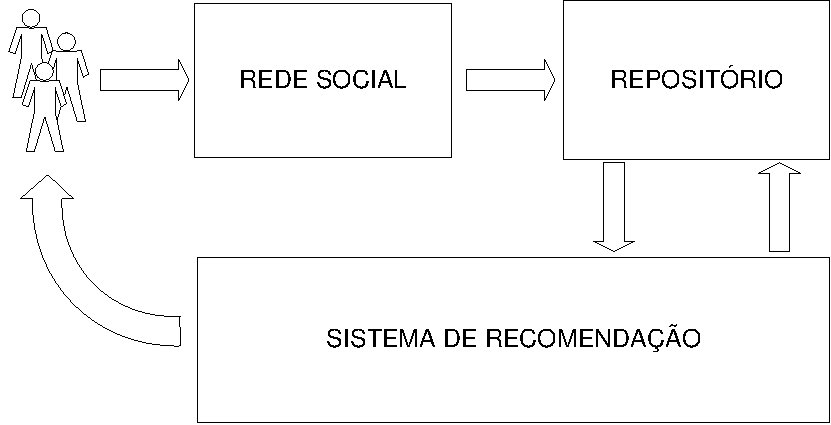
\includegraphics[width=\textwidth]{imagens/Diagrama_Visao_Geral}
  \caption{\it Diagrama de blocos do sistema}
  \label{fig:escopo}
\end{figure}

% section visao_do_sistema (end)

\section{Descrição do Sistema}

 Através do sistema os usuários poderão indicar o interesse em produtos e realizar recomendações a outros usuários. Quando um usuário avaliar um produto recomendado por outro o índice de confiança deste em relação ao outro é atualizado no sistema. Com base nas recomendações e nas avaliações o sistema irá inferir as seguintes informações:
 
\begin{itemize}

 \item Similaridade entre usuários

 \item Similaridade entre produtos

 \item Grau de confiança entre usuários

 \item Recomendações de produtos mais relevantes para um determinado usuário

\end{itemize}

 As recomendações geradas pelo sistema são baseadas nas avaliações de produtos feitas pelos usuários. A partir destas avaliações o sistema calcula a similaridade entre usuários, as relações de confiança e as relações encontradas entre os produtos.

  O usuário do sistema tem a opção de buscar os produtos já cadastrados através de uma ferramenta de busca incorporada à rede social. Além disso, os usuários podem recomendar os produtos para outros usuários presentes na rede social. Os usuários são informados que devem sempre realizar boas recomendações. Uma boa recomendação é a indicação de um produto que o outro usuário provavelmente terá o máximo interesse.

 Ao receber uma recomendação o usuário tem a opção de a avaliar o produto e então o sistema atualiza as informações relativas aos seus interesses. As avaliações de produtos são feitas em uma escala de 1 a 5, onde 1 representa que o usuário não tem nenhum interesse no produto, e 5 significa que o usuário tem muito interesse no produto. Estas informações são utilizadas para verificar a similaridade entre usuários, a similaridade entre itens e o índice de confiança.
 
 Quando um usuário avalia um produto recomendado por outro, essa avaliação altera o grau de confiança do usuário que recomendou o produto em relação àquele que recebeu a recomendação. Caso a avaliação seja positiva, a confiança do receptor aumenta, porém, caso a avaliação seja negativa, significa que o usuário que recebeu a recomendação não a aceitou como relevante, diminuindo o grau de confiança.

 Todas as informações sobre as avaliações são armazenadas no repositório para que o sistema de recomendação as consulte e seja capaz de realizar recomendações de outros produtos aos usuários. Esse é um dos propósitos do sistema de recomendação: mostrar ao usuário apenas informações relevantes. A Figura~\ref{fig:aspectos_funcionais} apresenta os diagrama de blocos dos aspectos do sistema e a relação entre eles.
 
\begin{figure}
 \centering
 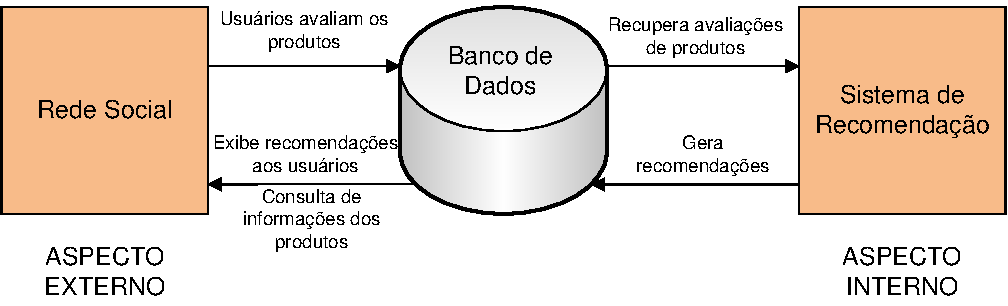
\includegraphics[width=\textwidth]{imagens/Implementacao_Detalhe2}
 \caption{\it Aspectos funcionais do sistema}
 \label{fig:aspectos_funcionais}
\end{figure}

\section{Funcionalidades principais} % (fold)
\label{sec:funcionalidades_principais}

Abaixo estão sumarizadas as principais funcionalidades do sistema acompanhadas das descrições em formato de \textit{user stories}\cite{557458}:

\begin{itemize}
  
  \item Envio de convite
  \subitem Como usuário, quero convidar outra pessoa a ingressar na rede social para que ela possa utilizar o sistema.
  
  \item Pedido de amizade
  \subitem Como usuário, quero convidar outro usuário a estabelecer uma relação de amizada na rede para que eu possa acompanhar as atividades dele na rede.
  
  \item Confirmação de amizade
  \subitem Como usuário, quero confirmar ou rejeitar um pedido de amizade para que eu possa acompanhar as atividades dos meus amigos pelo sistema.
	
	\item Avaliação de produto
  \subitem Como usuário, quero fazer a minha avaliação de produtos para que outros tenham conhecimento da minha opinião.
  
	\item Envio de recomendação de produto a outro usuário
  \subitem Como recomendador, quero enviar uma recomendação de produto para outra pessoa para que ela conheça a minha opinião sobre este item.
  
	\item Recomendação de produtos
	\subitem Como usuário, eu quero receber uma lista de produtos que eu provavelemente goste para que eu não precise filtrar os itens que me interessam.

    \item Visualização das avaliações dos usuários
    \subitem Como usuário, quero estar ciente sobre as últimas avaliações dos meus amigos para que eu possa saber o que acontece no meu contexto social e conheça novos produtos.
	
\end{itemize}

\section{Requisitos não-funcionais}

Os principais requisitos não-funcionais do sistema são:

\begin{itemize}

    \item Interface web compatível as últimas versões dos \textit{browsers} Internet Explorer, Mozilla Firefox e Safari.
    
    \item \textit{Backend} compatível com servidores Linux.

    \item Tempo médio de resposta menor que 2 segundos para 10 usuários simultâneos quando executado em um servidor com processador Intel Core 2 Duo T7250 ou superior e 2 GB de memória RAM. % esta é a configuração do meu notebook -- Allan

\end{itemize}

\section{Limites do Sistema}

\begin{itemize}
  
    \item O sistema não fará processamento de linguagem natural\footnote{\textit{Natural Language Processing (NLP)}}

\end{itemize}

\section{Implementação} % (fold)
\label{sec:implementacao}

A principal linguagem de programação utilizada no projeto foi Ruby, uma linguagem de script, com tipagem dinâmica, forte e implícita. Além disso, o Ruby permite uma abordagem multi-paradigma bem equilibrada entre os paradigmas orientado a objetos, funcional, imperativo e reflexivo. 

O \emph{framework} web Ruby on Rails foi escolhido para implementação do projeto. O Rails permite a adição de novas funcionalidades de forma ágil, pois é baseado em uma arquitetura \emph{Model-View-Controller}\cite{burbeck1992applications} (MVC) e segue os princípios \emph{Convention over Configuration}\cite{hansson2006convention} (CoC) e \emph{Don't Repeat Yourself}\cite{hunt-don} (DRY).

A lingugem Python também foi utilizada no projeto para algumas tarefas secundárias. Um script foi escrito nesta linguagem para fazer um \emph{crawler} e o \emph{parsing} de cerca de vinte mil produtos do site Submarino\footnote{www.submarino.com} para preencher a base de dados de produtos.

O SQLite é uma biblioteca independente que implementa um banco de dados SQL transacional, sem a necessidade de configurações. Este foi o gerenciador de banco de dados escolhido para o projeto, pois ele atende aos requistos de performance e facilita geração de backups.

Visando permitir um padrão de usabilidade aceitável para o usuário comum, algumas interações no sistema são realizadas via AJAX (Asynchronous JavaScript And XML). Através dessa técnica a aplicação pode obter dados do servidor de forma assíncrona sem interferir na apresentação e no comportamento da página atual. Esse recurso foi utilizado para permitir que os usuários registrassem o interesse em produtos sem que a página fosse totalmente recarregada. Como o uso dessa técnica requer utilização de JavaScript no \emph{browser} (cliente), e nem todos os \emph{browsers} tem JavaScript habilitado, o sistema tolera esse deficiência do cliente e possibilita neste caso o acesso através de uma requisição síncrona com recarregamento total da página.

A Figura~\ref{fig:rater-ajax} apresentar o painel de avaliação de produto que utiliza a técnica de AJAX. Ao clicar em uma das estrelas, uma requisição é enviada ao servidor para o cadastro da avaliação e, em caso de sucesso, a resposta enviada de volta ao \emph{browser} atualiza o estilo do elemento selecionado, indicando que a avaliação foi realizada.
\begin{figure}
 \centering
 
\includegraphics{imagens/rater-ajax}
 \caption{\it Avaliação de produto via AJAX}
 \label{fig:rater-ajax}
\end{figure}

O sistema conta com uma interface de administração na qual é possível enviar convites para novos usuários se integrarem a rede social. Quando um novo convite é gerado, automaticamente um \emph{token} pseudo-aletório é associado a ele. Esse \emph{token} é enviado através de e-mail, permitindo o registro apenas do convidado associado ao convite. A autenticação do usuário é feita através de login com e-mail e senha. O \emph{framework} escolhido para prover os mecanismos de autenticação foi o Warden\footnote{http://github.com/hassox/warden}, pois ele é adequado para oferecer poderosas opções de autenticação e pode ser utilizado em aplicações Rails através do Rack\footnote{http://rack.rubyforge.org/}.

A arquitetura cliente/servidor em três camadas, apresentada na Figura~\ref{fig:three_tier}, foi adotada na implementação do projeto. Essa escolha possibilita a modificação ou substituição de uma das camadas sem afetar as demais. Além disso, a separção entre as camadas de aplicação e de dados facilita o balanceamento da carga do sistema. Por fim, as políticas de segurança aplicadas no servidor podem ser rigorosas e, mesmo assim, não incomodar excessivamente os clientes.

\begin{figure}
 \centering
 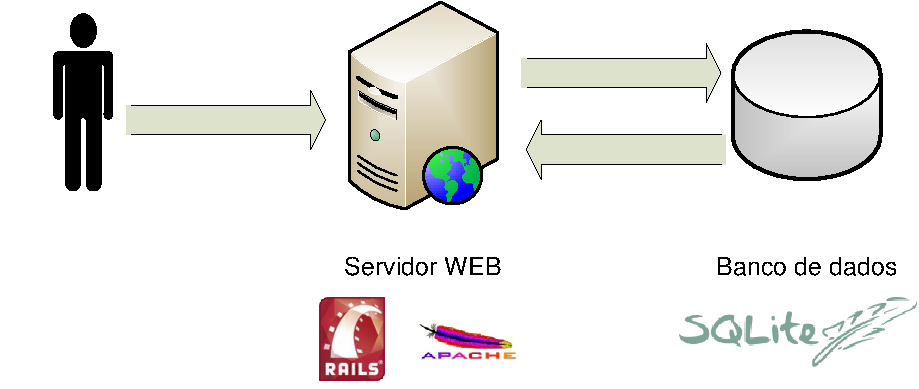
\includegraphics[width=\textwidth]{imagens/Implementacao_Detalhe}
 \caption{\it Arquitetura em três camadas}
 \label{fig:three_tier}
\end{figure}

% section implementacao (end)

% chapter especificacao_do_projeto (end)

\chapter{ESPECIFICAÇÃO DO EXPERIMENTO} % (fold)
\label{cha:especificacao_do_experimento} % (fold)

\section{Descrição do Experimento}
\label{cha:descricao_do_experimento}

Foi realizado um experimento com 60 pessoas, que se cadastraram e formaram uma rede social disposta em 12 grupos de 5 amigos. O sistema de recomendação utiliza essa rede social para obter as informações de relações de amizade entre as pessoas. Neste contexto, um participante é considerado amigo do outro quando eles pertencem a um mesmo grupo de amigos. Também foi levado em conta que dois amigos se conhecem, mantêm contato frequente e que têm noção dos seus interesses mútuos.

Inicialmente 12 pessoas foram convidadas para participarem do experimento e cada uma delas tinha a tarefa de montar o seu próprio grupo, convidando 4 amigos seus. Os grupos de amigos foram definidos a partir do envio de um e-mail com um convite do participante já cadastrado no sistema a outra pessoa. Este e-mail possuía um endereço de cadastro onde foi possível a pessoa se cadastrar e automaticamente já fazer parte do grupo de amigos do participante que a convidou.

Os participantes receberam recomendações dos seus amigos e de outras pessoas presentes na rede. Além disso, as informações de avaliações de produtos por parte dos participantes foram utilizadas pelo sistema de recomendação para recomendar outros produtos a eles. Como já citado no capítulo ~\ref{cha:introducao}, foram utilizados 3 tipos de algoritmos pelo sistema de recomendação:

\begin{itemize}
  \item Baseado em similaridade entre perfis
  \item Baseado em similaridade de produtos
  \item Baseado em confiança
\end{itemize}

Inicialmente 12 pessoas foram convidadas a participar do experimento. Cada uma destas convidou outras 4 pessoas para formarem um grupo de amigos. Sendo assim, formaram-se 12 grupos de 5 amigos, totalizando 60 pessoas. Cada participante de um grupo de amigos concorda em ser definido como amigo de todos no grupo, ou seja, todas as pessoas pertencentes a um mesmo grupo de amigos se conhecem e se consideram amigas. Cada participante do experimento recebeu, leu e assinou uma cópia do Termo de Consentimento Livre e Esclarecido (vide Apêndice~\ref{cha:TCLE}) concordando em participar do experimento.

Os participantes realizaram o cadastro informando os seguintes dados pessoais:

\begin{itemize}
  \item Nome
  \item Sexo
  \item Faixa etária (18-25, 26-30, 31-40, +40)
  \item Foto
\end{itemize}

O experimento consistia em 6 etapas, onde os participantes deveriam executar tarefas descritas no próprio sistema. As cinco primeiras etapas do experimento serviram para montar a base de dados necessária para a realização da sexta e última etapa, a qual utilizaria a base para rodar os algoritmos de recomendação e compará-los ao término do experimento.

\subsection{Primeira Etapa}
\label{cha:primeira_etapa}

Logo após a finalização do cadastro no sistema, a primeira etapa do experimento era iniciada. Ela consistia na avaliação de 20 produtos em comum a todos os participantes de todos os grupos. Esses produtos foram selecionados previamente, com o intuito de abranger os diferentes gostos de todos os participantes. Esta etapa foi necessária para que houvesse um \textit{rating overlap} no sistema, ou seja, para que todos os participantes avaliassem um mesmo conjunto de produtos. Com isso, foi possível calcular a similaridade de perfis entre todos os participantes da rede. Além disso, com esta etapa, resolve-se o problema dos \textit{coldstart users}, pois todos os participantes iniciam o uso do sistema ativamente.

Avaliar um produto significa dizer o quanto o participante considera aquele produto como relevante para si, ou seja, o quanto ele se interessa pelo produto. A avaliação é feita por meio da atribuição de uma nota de 1 a 5, sendo que 1 significa ausência de interesse e 5 representa muito interesse. Esse interesse não significa necessariamente uma atitude de compra. O objetivo dessa avaliação é saber realmente o interesse do participante, podendo representar cobiça ou curiosidade, além de admiração pelo produto. A interface de avaliação está apresentada na Figura~\ref{fig:product-rating}.

\begin{figure}[htp]
  \centering
  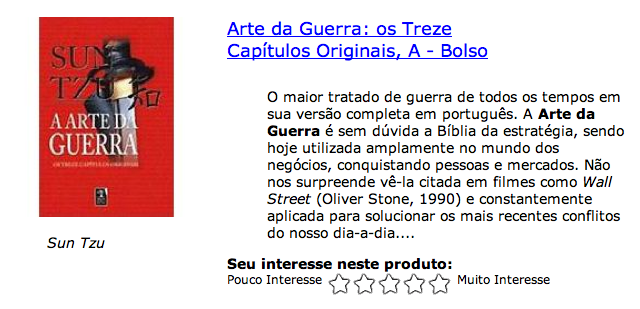
\includegraphics[width=\textwidth]{imagens/product-rating}
  \caption{\it Apresentação de produto para avaliação do participante}
  \label{fig:product-rating}
\end{figure}

Caso o participante não conhecesse o produto na hora de avaliá-lo, ou seja, não tivesse ouvido falar dele ou não tivesse conhecimento suficiente para reconhecê-lo, até o instante em que ele lhe foi apresentado, ele deveria informar isso ao sistema por meio de uma opção disponibilizada após a avaliação de cada produto. Mesmo não conhecendo, o participante avaliava o produto de acordo com o seu grau de interesse. Neste caso, a avaliação deveria ser feita apenas com base na foto e descrição do produto.

\subsection{Segunda Etapa}
\label{cha:segunda_etapa}

Ao finalizar a primeira etapa, automaticamente a segunda etapa era ativada. Esta visava conhecer os interesses particulares dos participantes. Para isso, foram disponibilizados vários produtos, separados nas diversas categorias, sendo que o participante deveria avaliar 10 produtos. As categorias escolhidas foram as seguintes:

\begin{itemize}
  \item CDs
  \item DVDs e Blu Ray
  \item Livros
  \item Livros Importados
  \item Celulares e Telefonia Fixa
  \item Vinhos e Bebidas
  \item Relógios e Presentes
  \item Informática e Acessórios
\end{itemize}

Os dados dos produtos foram retirados do site da Submarino\footnote{http://www.submarino.com}, sendo que apenas algumas categorias de livros, CDs e DVDs foram cadastradas no sistema e apenas os 60 produtos mais vendidos das outras categorias foram inseridos no cadastro.

Uma busca por nome foi implementada para que os participantes pudessem localizar um produto ao seu gosto e avaliá-lo. Nesta etapa, também estava disponível a opção de ``Não conheço'', pois era possível o participante encontrar durante a busca um produto desconhecido que o agradasse. A interface de busca de produtos está ilustrada na Figura~\ref{fig:product-search}.

Esta etapa era necessária para que os participantes avaliassem outros produtos além daqueles da primeira etapa que garantem o \textit{rating overlap}. Além dos produtos em comum, os sistemas de recomendação necessitam que as pessoas contribuam com informações individuais, pois um sistema de recomendação sempre indica produtos que não tenham sido avaliados pelo participante que receberá a recomendação. Desse modo, além das pessoas avaliarem produtos em comum, é necessário que elas avaliem diferentes produtos para que o sistema de recomendação tenha outros produtos a indicar.

\begin{figure}[htp]
  \centering
  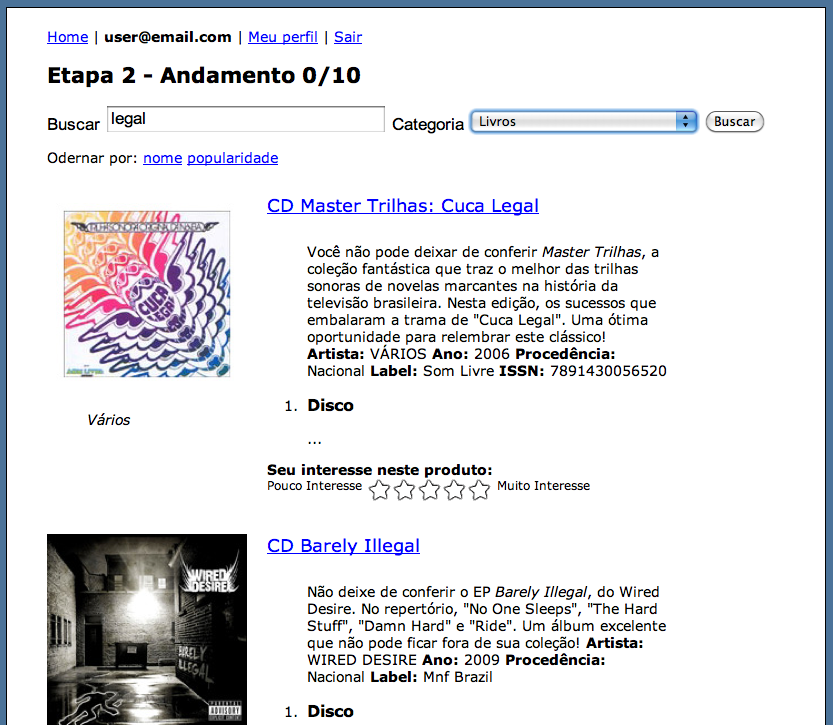
\includegraphics[width=\textwidth]{imagens/search}
  \caption{\it Interface de busca de produtos}
  \label{fig:product-search}
\end{figure}

\subsection{Terceira Etapa}

% TODO verificar tempo verbal no texto todo
Assim que todos os participantes terminassem as duas primeiras etapas do experimento, a terceira etapa era iniciada. Enquanto isso não ocorresse, quem terminava a segunda etapa recebia a mensagem do sistema informando que a terceira etapa estava desabilitada. Esse sincronismo foi necessário, pois as etapas seguintes necessitavam das informações de avaliação de produtos de todas as pessoas.

Nesta terceira etapa, o participante deveria recomendar produtos às pessoas do seu grupo. Como todos os integrantes de um grupo eram amigos entre si, era esperado que as recomendações de produtos fossem fáceis de serem realizadas, porque normalmente as pessoas conhecem os gostos dos amigos. Por isso, cada participante deveria recomendar 5 produtos a cada amigo, ou seja, 20 produtos no total.

A Figura~\ref{fig:stage-3} apresenta a interface do participante no início da etapa 3.

A busca de produtos estava disponível nesta etapa, bem como as avaliações de todos os amigos contendo no total os 30 produtos que cada um avaliou nas duas primeiras etapas do experimento. Não era possível um participante recomendar um produto já avaliado pela pessoa que receberia a recomendação, assim como não era possível recomendar o mesmo produto mais de uma vez para a mesma pessoa. Mesmo assim, o participante poderia receber duas recomendações de um mesmo produto, desde que elas fossem feitas por amigos diferentes. Neste caso o sistema armazenava as duas recomendações como distintas e mostrava apenas uma vez o produto para ser avaliado pela pessoa que recebeu a recomendação.

\begin{figure}[htp]
  \centering
  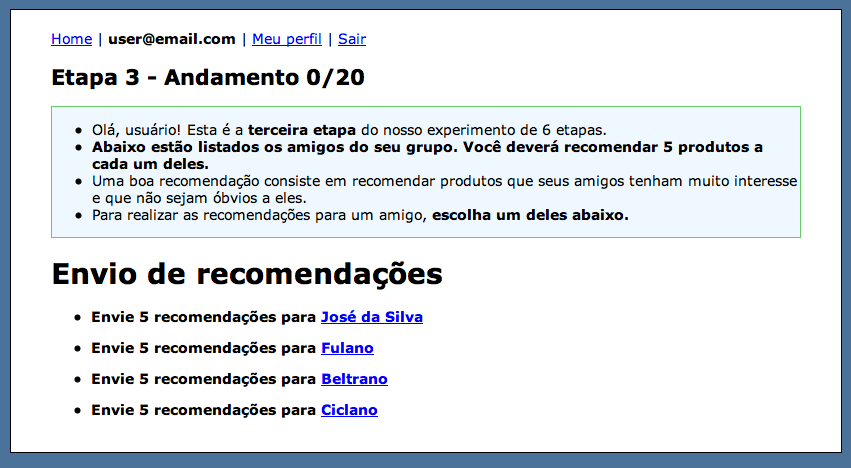
\includegraphics[width=\textwidth]{imagens/stage-3}
  \caption{\it Envio de recomendações de produtos}
  \label{fig:stage-3}
\end{figure}

Esta etapa era necessária para que posteriormente fosse possível analisar a eficiência da recomendação de produtos realizadas por amigos: nossa hipótese é que tal tipo de recomendação deveria ser mais eficiente do que as recomendações realizadas por pessoas desconhecidas ou pelo sistema de recomendação \cite{bonhard2007devil}.

\subsection{Quarta Etapa}

Depois de ter feito as 5 recomendações de produtos a cada amigo, o participante deveria recomendar alguns produtos a pessoas que não faziam parte do seu grupo, ou seja, pessoas desconhecidas. Ficava visível ao participante uma lista gerada pelo sistema contendo alguns desconhecidos. Tal lista foi gerada aleatoriamente em um aplicativo desenvolvido especialmente para este fim. Para cada pessoa na lista, o participante deveria recomendar apenas um produto. As avaliações de produtos realizadas por essas pessoas da lista ficavam disponíveis ao participante, sendo que ele deveria se basear apenas nestes dados e nos dados pessoais da pessoa para lhe recomendar um produto.

Com as recomendações realizadas por pessoas desconhecidas, foi possível comparar estas com aquelas feitas pelos amigos durante a terceira etapa do experimento. Foi necessário esperar todos os participantes terminassem a terceira e quarta etapas para que o experimento desse continuidade, já que todas essas recomendações de produtos seriam utilizadas nas etapas seguintes.

\subsection{Quinta Etapa}

A quinta etapa tinha como propósito mostrar apenas as recomendações diretas, ou seja, aquelas que foram feitas tanto pelos amigos do participante, como pelas pessoas desconhecidas. Os produtos recomendados eram listados ao participante para que ele os avaliasse novamente de acordo com o seu grau de interesse, além de informar se os conhecia ou não.

Na listagem de recomendações, não ficava visível ao participante quem lhe recomendou o produto, para que a origem da recomendação não tivesse nenhuma influência na hora de demonstrar o seu nível de interesse no produto. Caso estivesse exposto que um amigo seu lhe recomendou o produto, o participante poderia avaliá-lo bem só por causa do laço de amizade que tem com o recomendador. Ou, no caso contrário, avaliar mal um produto só porque não conhece a pessoa que o recomendou. Não havendo esse tipo de influência foi possível analisar as avaliações de produtos recomendados por amigos e desconhecidos de modo semelhante.

Para o sistema realizar as recomendações baseadas em confiança, era necessário que a terceira e quarta etapas fossem finalizadas por todos os participantes. Ao término da segunda etapa o sistema já poderia recomendar produtos, mas utilizando apenas os algoritmos baseados em perfil e em produto. A utilização desses algoritmos já era possível porque as avaliações dos 20 produtos da primeira etapa e a dos 10 da segunda já forneciam dados suficientes. Porém, como o algoritmo baseado em confiança necessita da avaliação de produtos recomendados diretamente por pessoas, foi decidido que todas as recomendações realizadas pelo sistema, a partir dos algoritmos baseados em perfil, produto e confiança, seriam realizadas ao término da quarta etapa. Com a avaliação dos produtos recomendados na terceira e quarta etapas os algoritmos baseados em perfil e em produto teriam mais dados para os seus cálculos.

Nenhum participante desistiu do experimento nesta etapa. No total, 51 participantes alcançaram a sexta e última etapa.

\subsection{Sexta Etapa}

A sexta etapa do experimento consistia na avaliação dos produtos recomendados pelo sistema aos participantes. Foram utilizados os 3 tipos de algoritmos para as recomendações, sendo que cada um deles originou 10 recomendações de produtos, totalizando 30 recomendações. Em alguns casos dois algoritmos diferentes recomendaram o mesmo produto. Quando isso ocorria, a recomendação era contabilizada normalmente para os dois algoritmos e o produto era mostrado apenas uma vez ao participante para ser avaliado.

\begin{table}
\centering
\begin{tabular}{c c c}
	\hline \hline
	\textbf{Etapa}	&	\textbf{Participantes que desistiram}	&	\textbf{Participantes que finalizaram}	\\
	\hline
	1	&	2	&	58	\\
	\hline
	2	&	2	&	56	\\
	\hline
	3	&	3	&	53	\\
	\hline
	4	&	2	&	51	\\
	\hline
	5	&	0	&	51	\\
	\hline
	6	&	1	&	50	\\
	\hline
\end{tabular}
\caption{\it Número de participantes durante as etapas do experimento}
\label{table:participantes}
\end{table}

Esta foi a etapa mais importante do experimento, pois é nela que se obteve os resultados das avaliações dos produtos recomendados com base na confiança. Além disso, houve também a avaliação dos produtos recomendados com base nos outros dois algoritmos, para que se pudesse analisar e comparar a eficiência dos três algoritmos utilizados no experimento.

Assim que os participantes terminavam as avaliações dos produtos, uma mensagem de agradecimento era mostrada e o experimento era finalizado.

Apenas um participante desistiu desta etapa final, totalizando 50 pessoas em um total de 60 a realizarem todas as etapas do experimento. A Tabela~\ref{table:participantes} mostra o número de participantes que realizaram as diferentes etapas do experimento e o número de participantes que desistiram do experimento durante as mesmas.
\chapter{ANÁLISES E RESULTADOS} % (fold)
\label{cha:analises_e_resultados}

\section{Introdução}
\label{cha:introducao}

 A análise dos resultados consistiu na elaboração de gráficos e tabelas com os dados retirados da base do experimento realizado. Os seguintes dados foram considerados para a análise:
 
\begin{itemize}
	\item Grupos de usuários
	
	\subitem Para se ter noção dos laços de amizades entre os participantes cadastrados no experimento. São 12 grupos no total, sendo que cada um deles possui no máximo 5 pessoas.
	
	\item Recomendações realizadas por amigos
	
	\subitem Informações dos produtos que foram recomendados na etapa 3 do experimento, onde os participantes deveriam recomendar 5 produtos a cada amigo presente no seu grupo. Cada participante possui no máximo 20 recomendações, sendo que alguns possuem apenas 15 devido à desistência de participantes do seu grupo.
	
	\item Recomendações realizadas por desconhecidos
	
	\subitem Informações dos produtos que foram recomendados na etapa 4 do experimento, onde os participantes deveriam recomendar 1 produto a alguns participantes de diferentes grupos, considerados desconhecidos. Cada participante possui no máximo 10 recomendações realizadas por desconhecidos, sendo que alguns possuem menos de 10 recomendações devido à desistência de participantes no experimento.
	
	\item Recomendações realizadas pelo sistema
	
	\subitem Todas as recomendações que o sistema realizou para os participantes. Contém a informação de qual participante recebeu a recomendação e qual foi o produto recomendado.
	
	\item Avaliação prevista do produto pelo sistema
	
	\subitem Ao recomendar um produto a um participante, o sistema calcula uma nota prevista para o mesmo. Essas informações foram armazenadas e consideradas durante a análise e exposição dos dados do experimento.
	
	\item Avaliações dos produtos
	
	\subitem Todas as avaliações de produtos no sistema. Contém os produtos avaliados na duas primeiras etapas do experimento, quando os participantes avaliaram 20 produtos em comum e 10 produtos de seu interesse, e as avaliações de produtos recomendados tanto pelos participantes como pelo sistema.
	
	\item Algoritmo utilizado para a recomendação
	
	\subitem Dentre as recomendações realizadas pelo sistema, foi retirada da base de dados a informação de qual algoritmo foi utilizado para gerar a recomendação.
	
\end{itemize}

 De posse dos dados, foram feitas as seguintes análises:
 
\begin{itemize}
	\item Análise Comparativa dos Algoritmos de Recomendação
	\item Análise de Rejeição das Recomendações
	\item Taxa de Serendipidade
	\item Análise do Algoritmo Baseado em Confiança
\end{itemize}

 Cada análise será discutida nas seções a seguir.
 
\section{Análise Comparativa dos Algoritmos de Recomendação}
\label{sec:analise_comparativa_dos_algoritmos_de_recomendacao}

Nesta seção serão comparados os resultados dos três algoritmos de recomendação e as recomendações diretas feitas tanto por amigos quanto por desconhecidos.

\begin{figure}
    \centering
    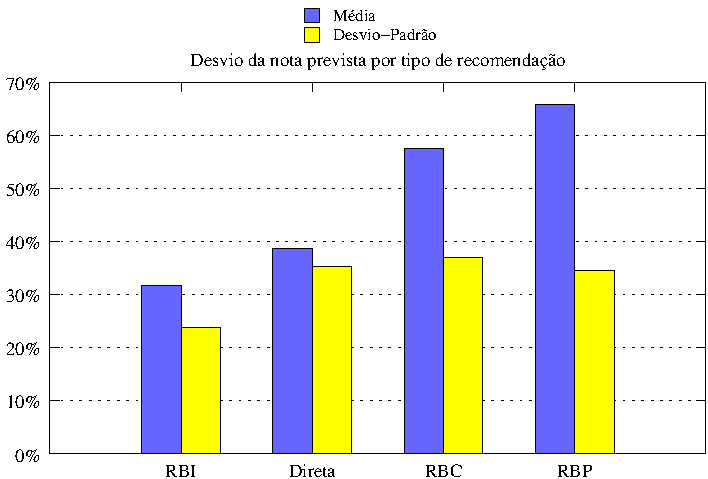
\includegraphics[width=\textwidth]{imagens/grafico_erro}
    \caption{\it Desvio da nota prevista por tipo de recomendação}
    \label{fig:erro}
\end{figure}

\begin{table}
\centering
\begin{tabular}{c c c}
    \hline \hline
    \textbf{Tipo de recomendação} & \textbf{Média}	& \textbf{Desvio-Padrão} \\
\hline 
Direta & 38.60\% & 35.23\% \\
\hline 
RBC & 57.40\% & 37.00\% \\
\hline 
RBI & 31.61\% & 23.75\% \\
\hline 
RBP & 65.80\% & 34.54\% \\
\hline        
\end{tabular}
\caption{\it Desvio da nota prevista por tipo de recomendação}
\label{table:erro}
\end{table}

A Figura~\ref{fig:erro} ilustra o desvio na nota prevista pelos tipos de recomendação. A Tabela~\ref{table:erro} contém os dados utilizados para a construção do gráfico. O desvio é a diferença entre a nota máxima esperada na recomendação e a nota realmente dada pelo participante. Os valores estão descritos em porcentagem em relação ao desvio máximo. A nota máxima prevista na recomendação é 5. Portanto, o desvio máximo é 4, pois a menor nota possível a ser dada é 1. O valor final apresentado é a média desses desvios.

Podemos verificar que o algoritmo RBI demonstrou o melhor desempenho, seguido das recomendações diretas, do algoritmo RBC e, por fim, do algoritmo RBP.

 As notas médias dadas pelos participantes estão discriminadas por algoritmos de recomendação e pelas recomendações diretas, como mostra a Figura~\ref{fig:notas_medias}. Os dados utilizados para a elaboração do gráficos estão na Tabela~\ref{table:notas_medias}. As recomendações que resultaram em uma média de notas maior foram as diretas, seguidas das realizadas com o algoritmo RBI, RBC e RBP.
 
\begin{figure}
    \centering
    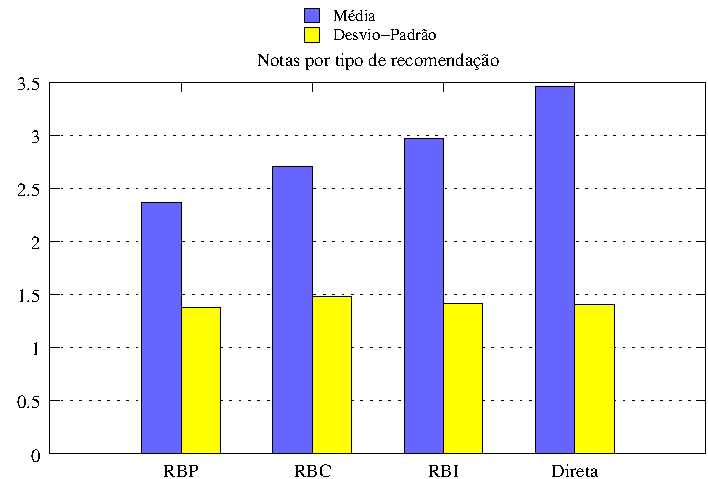
\includegraphics[width=\textwidth]{imagens/grafico_notas_medias}
    \caption{\it Notas por tipo de recomendação}
    \label{fig:notas_medias}
\end{figure}

\begin{table}
\centering
\begin{tabular}{c c c}
    \hline \hline
    \textbf{Tipo de recomendação} & \textbf{Média}& \textbf{Desvio-Padrão} \\
\hline 
Direta & 3.46 & 1.41 \\
\hline 
RBC & 2.70 & 1.48 \\
\hline 
RBI & 2.96 & 1.41 \\
\hline 
RBP & 2.37 & 1.38 \\
\hline        
\end{tabular}
\caption{\it Notas por tipo de recomendação}
\label{table:notas_medias}
\end{table}

 As notas médias dadas por recomendações diretas foram separadas entre as realizadas por amigos e as feitas por desconhecidos, como ilustra a Figura~\ref{fig:notas_medias_diretas}. Os dados utilizados para a construção do gráfico está na Tabela~\ref{table:notas_medias_diretas}. Verifica-se que a média de notas dadas por recomendações realizadas por amigos foi ligeiramente maior que as notas dadas a produtos indicados por desconhecidos.

\begin{figure}
    \centering
    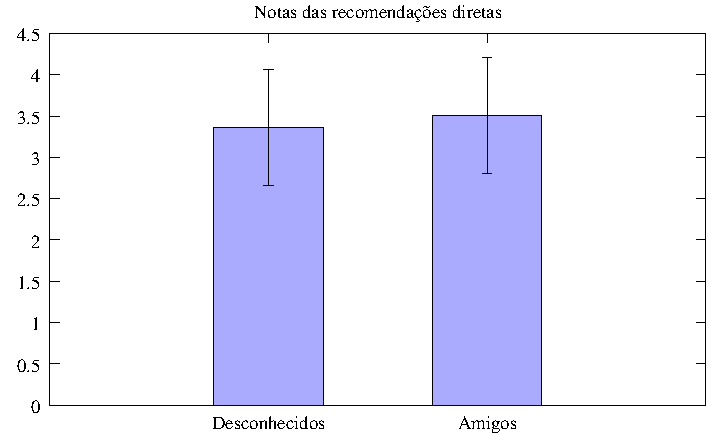
\includegraphics[width=\textwidth]{imagens/grafico_notas_medias_diretas}
    \caption{\it Notas das recomendações diretas}
    \label{fig:notas_medias_diretas}
\end{figure}

\begin{table}
\centering
\begin{tabular}{c c c}
    \hline \hline
    \textbf{Tipo de recomendação} & \textbf{Média}& \textbf{Desvio-Padrão} \\
\hline 
Amigos & 3.51 & 1.41 \\
\hline 
Desconhecidos & 3.36 & 1.40 \\
\hline        
\end{tabular}
\caption{\it Notas das recomendações diretas}
\label{table:notas_medias_diretas}
\end{table}

% section analise_comparativa_dos_algoritmos_de_recomendacao (end)

\section{Análise de Rejeição das Recomendações}
\label{sec:analise_de_rejeicao_das_recomendacoes}

 Nesta seção serão analisadas a taxa de rejeição das recomendações realizadas pelos algoritmos RBI, RBP e RBC, além das recomendações diretas. Para isso, foram definidas classes de avaliações. As avaliações com notas 1 e 2 são da classe de \textit{Rejeição}, as com nota 3 são da classe \textit{Indiferente} e as com notas 4 e 5 são da classe \textit{Aceitação}. A classe Rejeição denota as recomendação que não foram aceitas e a classe Aceitação denota as recomendações que foram aceitas. Na classe Indiferente estão as recomendações que tiveram avaliações neutras (nota 3).

 Podemos verificar pela Figura~\ref{fig:notas} que as recomendações diretas representaram uma maior porcentagem de notas na classe de Aceitação, seguida das recomendações feitas pelo algoritmo RBI, RBC e, por fim, RBP. Os dados utilizados para a elaboração do gráfico constam na Tabela~\ref{table:notas}.
%TODO concluir análise
 
\begin{figure}
    \centering
    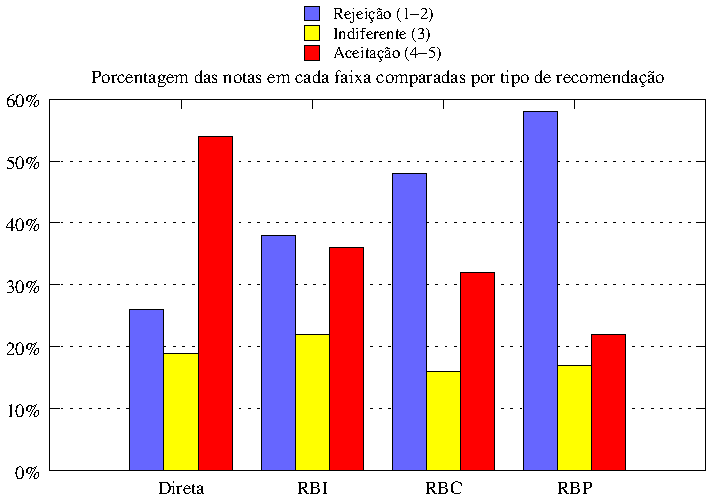
\includegraphics[width=\textwidth]{imagens/grafico_notas}
    \caption{\it Porcentagem das notas em cada faixa comparadas por tipo de recomendação}
    \label{fig:notas}
\end{figure}

\begin{table}
\centering
\begin{tabular}{c c c c} 
    \hline \hline
    \textbf{Tipo de recomendação} & \textbf{Rejeição}& \textbf{Indiferente}& \textbf{Aceitação} \\
\hline 
Direta & 26\% & 19\% & 54\% \\
\hline 
RBC & 48\% & 16\% & 32\% \\
\hline 
RBI & 38\% & 22\% & 36\% \\
\hline 
RBP & 58\% & 17\% & 22\% \\
\hline        
\end{tabular}
\caption{\it Porcentagem das notas em cada faixa comparadas por tipo de recomendação}
\label{table:notas}
\end{table}

% section analise_de_rejeicao_das_recomendacoes (end)

\section{Taxa de Serendipidade}
\label{sec:taxa_de_serendipidade}

Serendipidade significa o usuário ter aceitado a recomendação, ou seja, ter dado uma nota 4 ou 5 ao produto e não o conhecer. A taxa de serendipidade foi calculada com base no número de recomendações de produtos desconhecidos aceitas sobre o total de produtos recomendados em cada tipo de algoritmo, considerando também as recomendações diretas. A Figura~\ref{fig:serendipidade} mostra a taxa de serendipidade para os tipos de recomendação, sendo que os dados utilizados para elaborar o gráfico estão na Tabela~\ref{table:serendipidade}.

Verificamos que as recomendações diretas resultaram em um alto grau de serendipidade, se comparado com os graus dos tipos de recomendações que as seguiram: RBI, RBC e RBP.

\begin{figure}
    \centering
    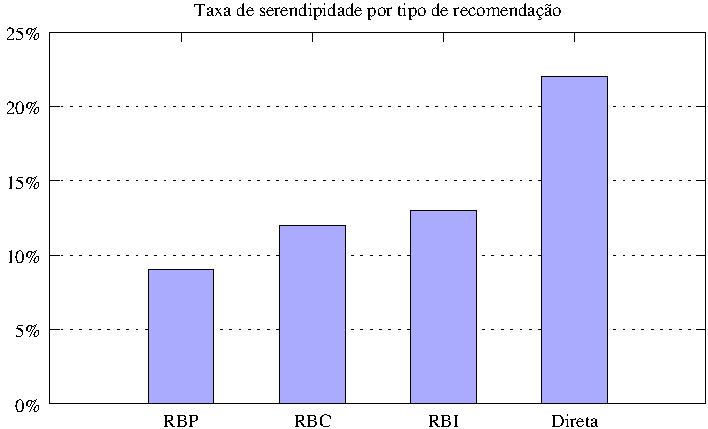
\includegraphics[width=\textwidth]{imagens/grafico_serendipidade}
    \caption{\it Taxa de serendipidade por tipo de recomendação}
    \label{fig:serendipidade}
\end{figure}

\begin{table}
\centering
\begin{tabular}{c c}
    \hline \hline
    \textbf{Tipo de recomendação} & \textbf{Taxa de Serendipidade} \\
\hline 
Direta & 22\% \\
\hline 
RBC & 12\% \\
\hline 
RBI & 13\% \\
\hline 
RBP & 9\% \\
\hline        
\end{tabular}
\caption{\it Taxa de serendipidade por tipo de recomendação}
\label{table:serendipidade}
\end{table}

A Figura~\ref{fig:serendipidade_diretas} compara a taxa de serendipidade entre as recomendações diretas realizadas por amigos e por desconhecidos. A Tabela~\ref{table:serendipidade_diretas} contém os dados utilizados para elaborar o gráfico. Podemos ver que as recomendações realizadas pelos amigos resultaram em uma taxa de serendipidade ligeiramente maior que as recomendações realizadas por desconhecidos.
%TODO concluir análise

\begin{figure}
    \centering
    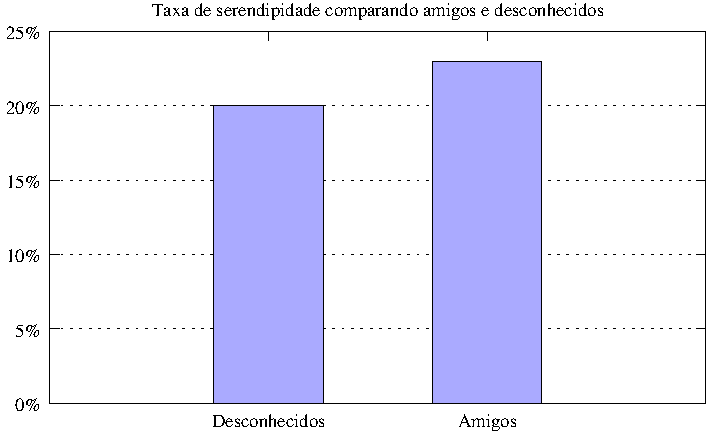
\includegraphics[width=\textwidth]{imagens/grafico_serendipidade_diretas}
    \caption{\it Taxa de serendipidade comparando amigos e desconhecidos}
    \label{fig:serendipidade_diretas}
\end{figure}

\begin{table}
\centering
\begin{tabular}{c c}
    \hline \hline
    \textbf{Tipo de recomendação} & \textbf{Taxa de Serendipidade} \\
\hline 
Amigos & 23\% \\
\hline 
Desconhecidos & 20\% \\
\hline        
\end{tabular}
\caption{\it Taxa de serendipidade comparando amigos e desconhecidos}
\label{table:serendipidade_diretas}
\end{table}

% section taxa_de_serendipidade (end)

\section{Análise do Algoritmo Baseado em Confiança}
\label{sec:analise_do_algoritmo_baseado_em_confianca}

 Com os dados apresentados na seções anteriores, podemos verificar que o algoritmo de recomendação baseado em confiança (RBC) possuiu resultados relativamente bons principalmente com relação ao RBP.
 
 Na análise de desvio da nota prevista o RBC não foi tão eficiente quanto as recomendações diretas e o algoritmo RBI, porém mostrou resultados melhores que o RBP. 
 
 Verificando a média de notas dadas, o RBC teve resultado intermediário com relação aos outros dois algoritmos, sendo que as recomendações diretas apresentaram a melhor eficiência. Isso ocorreu principalmente pelo fato dos desconhecidos terem recomendado quase tão bem como os amigos, como mostra a Figura~\ref{fig:notas_medias_diretas}.
 
 Quanto à taxa de serendipidade, o RBC manteve-se na média dos outros algoritmos, sendo que as recomendações diretas foram disparadamente mais eficientes.
 
 De acordo com os dados, o RBC conseguiu recomendar melhor que o RBP, que é o algoritmo que o RBC se baseia para recomendar. O RBC utiliza menos informações que o RBP para recomendar e mesmo assim mostrou-se melhor nos resultados do experimento.

% section analise_do_algoritmo_baseado_em_confianca (end)

\section{Análise das Hipóteses}

Um dos objetivos do experimento foi testar certas hipóteses que, ao serem confirmadas, fornecem uma base mais sólida para a construção de sistemas de recomendação efetivos.

A seguir cada hipótese será analisada. As hipóteses nulas (H0) são todas iguais, elas consideram que as duas diferentes distribuições pouco diferem, tendo por exemplo a mesma média, mediana ou algum critério equivalente que depende exatamente do teste de hipótese utilizado. Para mais informações, consultar a seção apêndice~\ref{anexo_hipoteses}, onde estão listados os testes utilizados e os resultados numéricos dos mesmos.

\subsection{Os amigos recomendam melhor do que os desconhecidos}
A hipótese nula foi rejeitada com um nível de significância de 10\%, confirmando esta hipótese quando também se considera que a média das recomendações dos amigos é maior do que as dos desconhecidos, conforme pode ser visto na figura~\ref{fig:notas_medias_diretas}.


\subsection{A recomendação baseada em confiança é melhor do que a baseada em similaridade de perfil dos usuários}
A hipótese nula foi rejeitada com um nível de significância de 0.5\%, confirmando a hipótese de que o algoritmo apresentado nesta monografia (RBC) é superior ao algoritmo de similaridade de perfil (RBP) que é um dos mais utilizados na filtragem social. As figuras \ref{fig:notas} e \ref{fig:notas_medias} mostram a melhor aceitação da RBC em relação a RBP.


\subsection{Hipóteses secundárias}

\subsubsection{As recomendações diretas são melhores do que as RBC}
A hipótese nula foi rejeitada com um nível de significância de 0.5\%, confirmando que as recomendações feitas diretamente pelas pessoas possuem uma aceitação muito maior do que o algoritmo apresentado neste trabalho, como pode ser visto nas figuras~\ref{fig:notas} e \ref{fig:notas_medias}.

\subsubsection{As recomendações baseadas em similaridade de itens são melhores do que as baseadas em confiança}
A hipótese nula foi rejeitada com um nível de significância de 0.5\%, confirmando, como pode ser visto nas figuras \ref{fig:notas} e \ref{fig:notas_medias}, que a RBI é melhor aceita do que a RBC.


\section{Análise de Desempenho}
\label{sec:analise_de_desempenho}
% TODO falar sobre os problemas enfrentados com as consultas SQL e com as estrelinhas para a avaliação do produto (javascript).

Durante a realização do experimento algumas requisições ao servidor de aplicação foram identificadas como gargalo de desempenho do sistema. Ao analisar estas requisições, foi possível verificar que o fatores responsáveis pela degradação da performance estavam relaciondos ao tempo e quantidade das requsições ao banco de dados. As consultas SQL na tabela de produtos, com cerca de cento e vinte mil registros, foram as principais responsáveis pelo aumento no tempo de resposta. Esses problemas de performance foram rapidamente corrigidos através da redução do número de requisições ao banco de dados e pela paginação dos resultados. Os tempos de resposta das requisições antes da otmização das consultas podem ser observados na Tabela~\ref{table:before_stats} e comparados com os valores obtidos após a otmização na Tabela~\ref{table:after_stats}.

\begin{table}\centering
\begin{tabular}{c c c c c}
\hline \hline
\textbf{Requisição Web}
& \textbf{Média}
& \textbf{Desvio Padrão}
& \textbf{Min.} 
& \textbf{Max.} \\ \hline
ProductsController\#index.html [GET]    & 16.90s & 29.02s &  0.00s &  5m06s \\
\hline
ProductsController\#rate.html [POST]    &  2.09s &  1.24s &  0.80s & 32.16s \\
\hline
ProductsController\#unknown.html [POST] &  1.26s &  0.54s &  0.85s &  2.42s \\
\hline
ProductsController\#show.html [GET]     &  1.18s &  1.21s &  0.00s &  8.52s \\
\hline
\end{tabular}
\caption{\it Tempo de resposta das requisições ao banco de dados antes da otimização \label{table:before_stats}}
\end{table}

\begin{table}\centering
\begin{tabular}{c c c c c}
\hline \hline
\textbf{Requisição Web}
& \textbf{Média}
& \textbf{Desvio Padrão}
& \textbf{Min.} 
& \textbf{Max.} \\ \hline
ProductsController\#index.html [GET]    & 1.28s &  3.51s &  0.00s & 57.42s \\
\hline
ProductsController\#rate.html [POST]    & 0.13s &  0.77s &  0.00s & 21.05s \\
\hline
ProductsController\#unknown.html [POST] & 0.02s &  0.10s &  0.00s &  2.66s \\
\hline
ProductsController\#show.html [GET]     & 0.02s &  0.12s &  0.00s &  1.99s \\
\hline
\end{tabular}
\caption{\it Tempo de resposta das requisições ao banco de dados após a otimização \label{table:after_stats}}
\end{table}

Para completar a análise da performance do sistema, a Tabela~\ref{table:process_blockers} apresenta as requisições bloqueantes, isto é, aquelas com duração total maior do que um segundo. Os dados apresentados na Tabela~\ref{table:process_blockers} são referentes apenas as requisições feitas após a otimização até o término do experimento.

\begin{table}\centering
\begin{tabular}{c c c}
\hline \hline
\textbf{Requisição Web}
& \textbf{Ocorrências}
& \textbf{Porcentagem} \\ \hline
UserRecommendationsController\#new.html [GET]     & 1596 & 65.2\% \\ 
\hline
ProductsController\#index.html [GET]              &  315 & 12.9\% \\ 
\hline
AdminController\#index.html [GET]                 &  167 &  6.8\% \\
\hline
ProductsController\#rate.html [POST]              &  165 &  6.7\% \\
\hline
HomeController\#index.html [GET]                  &  128 &  5.2\% \\ 
\hline
UserRecommendationsController\#create.html [POST] &   38 &  1.6\% \\
\hline
RecommendationGuidesController\#index.html [GET]  &   11 &  0.4\% \\  
\hline
InvitationsController\#create.html [POST]         &    8 &  0.3\% \\  
\hline
ProductsController\#unknown.html [POST]           &    8 &  0.3\% \\  
\hline
RatingsController\#index.html [GET]               &    7 &  0.3\% \\  
\hline
SessionsController\#create.html [POST]            &    4 &  0.2\% \\  
\hline
UsersController\#new.html [GET]                   &    1 &  0.0\% \\  
\hline
ProductsController\#show.html [GET]               &    1 &  0.0\% \\
\hline
\end{tabular}
\caption{\it Requisições bloqueantes \label{table:process_blockers}}
\end{table}


% section analise_de_desempenho (end)

\chapter{CONSIDERAÇÕES FINAIS} % (fold)
\label{cha:consideracoes_finais}

\section{Trabalhos Futuros}
\label{sec:trabalho_futuros}

 Nesta seção serão descritos possíveis trabalhos futuros relacionados ao que foi realizado neste projeto. Alguns deles não puderam ser implementados devido às restrições de tempo ou por mudança no escopo do projeto.

\subsection{Web Semântica} % (fold)
\label{sub:web_semantica}

 A World Wide Web é um sistema de documentos em hipermídia que são interligados e executados na Internet. A maioria do conteúdo disponível na Web atualmente é projetado para a leitura por seres humanos. A utilização de programas de computador para interpretação desse conteúdo é complexa devido à baixa flexibilidade dos programas em relação aos humanos. Se por um lado os aplicativos são menos flexíveis que os seres humanos para interpretação de textos, por outro eles são capazes de desenvolver e analisar estruturas de dados complexas. A Web Semântica baseia-se nessa virtude do software. 

 Segundo Berners-Lee \cite{bemerslee2001sw}, a Web Semântica não é uma Web separada, mas um extensão da atual, na qual a informação é disponibilizada com sentido bem definido, aprimorando a capacidade de cooperação entre pessoas e computadores. Os documentos nesta extensão da Web são convenientes para utilização tanto por humanos como por programas.

 Da mesma forma que os humanos buscam informações em bases de dados descentralizadas na Web, com a adoção da Web Semântica agentes computacionais poderão fazer o mesmo. Essa descentralização de documentos permite que inconsistências ocorram, porém possibilita um rápido crescimento no volume de dados.

 A W3C realiza trabalhos para aprimorar, entender e padronizar a Web. Com o apoio de uma equipe especializada do consórcio, tecnologias para representação estrutural e semântica dos recursos na Web foram desenvolvidas, resultando em um conjunto de especificações para a Web Semântica. Atualmente este conjunto é basicamente composto pelo Resource Description Framework (RDF), a linguagem RDF Schema e a Web Ontology Language (OWL).

 Os mecanismos de busca atualmente utilizados na Web são capazes de listar os sites que contenham os termos desejados, bem como ordená-los de acordo com critérios de relevância. Considerando as dificuldades impostas à interpretação do conteúdo pelos computadores, fica a cargo do usuário a tarefa de identificar quais dos sites obtidos são coerentes com as expectativas de contexto e necessidade.

 Cientes disso, o grupo tinha proposto inicialmente um sistema de recomendação baseado em confiança com padrões da web semântica. Todas as informações contidas no repositório seriam documentos semanticamente estruturados em padrões abertos. Com isso, todas as informações sobre avaliações e recomendações de produtos, além de perfis de usuários estariam disponíveis para importação por outros sistemas que entendem a linguagem adotada nesses documentos. Desse modo, a filtragem e localização de produtos mais relevantes aos usuários ganharia a poderosa ferramenta do processamento computacional.

% subsection web_semantica (end)

\subsection{Confiança Dependente do Tempo} % (fold)
\label{sub:confianca_dependente_do_tempo}

 Em \cite{sabater2001regret} o modelo de reputação proposto é baseado no cálculo do parâmetro de reputação a partir da somatória dos pesos de impressões que o usuário tem de determinada entidade. Porém, o artigo levanta um ponto importante e crucial no modelo: a reputação ser dependente do tempo. Impressões antigas não podem ser consideradas com o mesmo peso das mais recentes. Para isso, os autores propuseram a utilização de uma função dependente do tempo tal como a Equação~\ref{eq:REGRET}.
 
\begin{equation}
 R^t(IDB_a) = {\sum_{t_i\in{IDB_a}}}\rho(t,t_i)\times{W_i}
 \label{eq:REGRET} 
\end{equation}

 Onde $R^t(IDB_a)$ significa a reputação no tempo $t$ que o agente $a$ tem da impressão $IDB$ \textit{Impressions Database}. Os pesos das impressões são os $W_i$, que são multiplicados por $\rho(t,t_i)$ e somados para todas as impressões que o agente tem. A função $\rho(t,t_i)$ é uma função dependente do tempo, como visto na Equação~\ref{eq:rho_t}.
 
\begin{equation}
 \rho(t,t_i) = \frac{f(t_i,t)}{{\sum_{t_j\in{IDB_a}}}f(t_j,t)}
 \label{eq:rho_t} 
\end{equation}

 A função $f(t_i,t)$ dá valores próximos de t, podendo ser a função $f(t_i,t) = \frac{t_i}{t}$. Com isso, impressões antigas não têm o mesmo peso que impressões mais recentes.

 Considerando o nosso sistema proposto, o cálculo da confiança entre dois usuários poderia levar em conta o tempo em que as avaliações dos produtos recomendados foram feitas. Isso porque o usuário pode avaliar mau um produto sem conhecê-lo, apenas demonstrando o seu baixo interesse nele. Após alguns meses, o usuário pode vir a conhecer o produto e passar a ter interesse no mesmo. Com isso, a sua avaliação antiga não estaria condizente com o seu gosto atual.
 
 O grupo não realizou a implementação desse modelo de confiança devido às restrições de tempo para a realização do experimento.

% subsection confianca_dependente_do_tempo (end)

\subsection{Feedback das Recomendações} % (fold)
\label{sub:feedback_das_recomendacoes}

 O conteúdo de uma rede social é tão bom quanto a qualidade da informação compartilhada pelos seus usuários. Novos usuários muitas vezes não entendem o valor dessa contribuição e entram em uma rede apenas para observar os outros e não inserir nenhuma informação ou opinião sua de qualidade. Por isso, a motivação para que novos entrantes ajudem na elaboração do conteúdo da rede social é muito importante e um dos meios para que isso ocorra é o \textit{feedback} que o usuário ganha ao contribuir com algo\cite{burke2009fmm}.
 Desse modo, quando um usuário compartilha alguma informação ele quer saber o que os outros presentes na rede acharam. Esse \textit{feedback} motiva os usuários a compartilharem cada vez mais e, com isso, aumentar o conteúdo presente na rede.
 A proposta de trabalho futuro envolve a adição de \textit{feedbacks} aos usuários que avaliarem ou recomendarem produtos na rede social. O sistema pode mostrar quais amigos do usuário avaliaram o mesmo produto ou simplesmente mostrar a avaliação que uma pessoa deu a um produto recomendado pelo usuário. De acordo com\cite{burke2009fmm}, essa informação de retorno que o sistema dá a um usuário que contribui na rede motiva o mesmo a continuar compartilhando informações.
 Esses mecanismos de \textit{feedback} não foram implementados no sistema utilizado no experimento para que os participantes não tivessem nenhuma influência na hora de avaliar ou recomendar os produtos. Caso o participante recebesse informações de retorno do sistema com relação às suas ações no experimento, ele poderia tentar mudar a sua estratégia de recomendação ou avaliação de produtos e, desse modo, não se comportar na sua maneira natural de agir.

% subsection feedback_das_recomendacoes (end)

%section trabalhos futuros (end)

\section{Conclusão}
\label{conclusao}

% section conclusao (end)

% chapter trabalhos_futuros (end)

\addcontentsline{toc}{chapter}{Referências Bibliográficas}
\bibliographystyle{abnt-num}   %\bibliographystyle{plain}
\bibliography{capitulos/bibliografia} % bibname=nome do seu arquivo BibTeX
\begin{thebibliography}{99}

 

%  \bibitem{marketing_social_web}
%    WEBER, LARRY.
%    \textbf{Marketing to the social web}: how digital customer communities build your business.
%    Wiley, 2007, 5 p.

\end{thebibliography}


%\addcontentsline{toc}{chapter}{Glossário}
%\chapter*{Glossário} % (fold)
\label{cha:glossario}

\begin{itemize}

  \item \emph{ADSL}: acrônimo de \emph{Asymmetric Digital Subscriber Line}, é uma forma de transmissão de dados de alta velocidade utilizando linhas telefônicas comuns, em freqüências maiores que os seres humanos conseguem escutar.

  \item \emph{BNC}: é um tipo de conector cujo nome vem de seus criadores: ``bayonet Neil-Concelman''. Sua grande característica é o sistema de trava, tipo twist-lock (gira e trava), que possibilita grande segurança na conexão. É bastante utilizado nos equipamentos profissionais de vídeo.

  \item \emph{Broadcast}: é um modo de difusão de sinais em que é transmitido o mesmo conteúdo para todos os receptores. Numa transmissão de TV, por exemplo, todas as pessoas sintonizadas no mesmo canal assistem ao mesmo programa. Em Internet, o termo é usado muitas vezes para designar o envio de uma mensagem par todos os membros de um grupo, em vez da remessa para membros específicos.

  \item \emph{Buffer}: é uma área de armazenamento que compensa diferentes velocidades de fluxos de dados ou temporizações de eventos, ao transferir dados de um dispositivo para outro.

  \item \emph{CD}: acrônimo de Compact Disc, é um padrão de armazenamento óptico para dados digitais.
  Conversor A/D: um Conversor Analógico-Digital é componente de um sistema responsável por converter dados analógicos para digitais através da amostragem de um sinal contínuo e sua posterior discretização gerando valores numéricos digitais.

  \item \emph{Classpath}: é um argumento passado para a Java Virtual Machine indicando onde procurar classes e pacotes para carregamento dinâmico.

  \item \emph{CPqD}: {C}entro de {P}es{q}uisa e {D}esenvolvimento em Telecomunicações.

  \item \emph{DivX}: é um formato de compactação de vídeo criado pela DivxNetworks Inc.

  \item \emph{Driver}: um driver é um componente de software responsável por estabelecer a comunicação entre hardware e software, provendo comandos para enviar e receber dados de um dispositivo instalado.

  \item \emph{DVD}: acrônimo de Digital Versatile Disc, é a geração seguinte ao CD, possibilitando um armazenamento maior de dados.

  \item \emph{ECMAScript}: é uma linguagem de programação baseada em scripts, padronizada pela Ecma International na especificação ECMA-262. A linguagem é bastante usada em tecnologias para Internet, sendo esta base para a criação do JavaScript/JScript e também do ActionScript.

  \item \emph{FIFO}: acrônimo para {F}irst {I}n, {F}irst {O}ut (que em português significa primeiro a entrar, primeiro a sair) refere-se a estruturas de dados do tipo fila onde os elementos vão sendo colocados e retirados (ou processados) por ordem de chegada.

  \item \emph{GEM}: acrônimo de \emph{Globally Executable MHP} \cite{gem}, é uma parte do MHP independente dos padrões de transmissão europeus, criado com a finalidade de padronizar partes de todos os padrões de \emph{middleware} mundiais e possibilitar a criação de aplicações que funcionem em qualquer \emph{middleware} que seja compatível com o GEM.

  \item \emph{GSM}: acrônimo de Global System for Mobile Communications é um dos principais padrões para telefonia móvel existente.

  \item \emph{Heap}: Heap de objetos é o nome dado a parte da memória do computador que contém a estrutura de dados responsável por armazenar todos os objetos durante a execução da máquina virtual Java.

  \item \emph{HTTP}: acrônimo para {H}yperText {T}ransfer {P}rotocol (Protocolo de Transferência de Hipertexto), utilizado para transferência de dados na rede mundial de computadores, a World Wide Web.

  \item \emph{IPC (Inter-Process Communication)}: é o grupo de mecanismos que permite aos processos transferirem informação entre si. Entre estes mecanismos podem ser citados pipes, filas de mensagens e memória compartilhada.

  \item \emph{Java}: é uma linguagem de programação orientada a objeto desenvolvida na década de 90 pelo programador James Gosling, na empresa Sun Microsystems.

  \item \emph{JavaBeans}: são componentes reutilizáveis de software escritos em linguagem Java, e que seguem algumas convenções de modo a permitir que ferramentas possam utilizá-los e manipulá-los.

  \item \emph{JavaTV}: é uma biblioteca Java que contempla a maior parte dos recursos necessários para a operação de sistemas receptores de TV digital, simplificando assim o desenvolvimento de softwares, uma vez que os programadores de aplicativos podem se voltar ao tema principal da aplicação em desenvolvimento.

  \item \emph{JNI (Java Native Interface)}: é um padrão de programação que permite que a máquina virtual da linguagem Java acesse bibliotecas construídas com o código nativo de um sistema.

  \item \emph{Lista ligada}: é uma estrutura de dados linear e dinâmica composta por células que apontam para o próximo elemento da lista.

  \item \emph{Metodologia (Processo) de Desenvolvimento Ágil}: metodologias de desenvolvimento ágil foram pensadas de forma a minimizar riscos no desenvolvimento de software através períodos mais curtos de lançamento, chamados iterações, que tipicamente levam de uma quatro semanas. Métodos ágeis prezam mais a comunicação face-a-face que a documentação, como forma de acelerar o processo de desenvolvimento.

  \item \emph{MHP}: acrônimo de \emph{Multimedia Home Platform} \cite{mhp}, é um padrão aberto de \emph{middleware} para TV Digital, adotado principalmente pelos países europeus. Está incluso em outro padrão maior, o \emph{Digital Video Broadcasting} (DVB) \cite{dvb} que agrupa todas as características da tecnologia de TV Digital européia.

  \item \emph{Middleware} (conforme \cite{ginga}): é a camada de software intermediário que permite o desenvolvimento de aplicações interativas para a TV Digital de forma independente da plataforma de hardware dos fabricantes de terminais de acesso (\emph{set-top boxes}).

  \item \emph{MPEG}: acrônimo para {M}oving {P}icture {E}xperts {G}roup, é o grupo de trabalho da Organização Internacional para Padronização (ISO) para o desenvolvimento de padrões para vídeo e áudio digitais.

  \item \emph{MPEG2}: é um padrão de compressão e codificação de vídeo para difusão e comunicações, bem como para armazenamento em meios diversos, tais quais os ópticos.

  \item \emph{MPEG-TS}: MPEG {T}ransport {S}tream (TS, TP, ou MPEG-TS) é um protocolo de  comunicação para transmissão de áudio, vídeo e dados, especificado pelo padrão  ISO/IEC 13818-1. Permite multiplexar vídeo e áudio digital sincronizando a saída. Possui correção de erro e transporte, e é usado para difusão de aplicações como DVB e ATSC.

  \item \emph{MOV}: formato de vídeo criado pela Apple, é um container para imagem, diversas trilhas, efeitos e textos. Sua base foi aprovada pela ISO como padrão para MPEG4 Part. 14.

  \item \emph{Multiplexação no tempo}: a multiplexação no tempo consiste na transmissão de dois ou mais sinais ou fontes de bits simultaneamente através de um único canal pela divisão do tempo em pequenos compartimentos de tamanhos fixos, onde são transmitidos alternadamente um pouco de cada sinal.

  \item \emph{Overhead}: Em computação overhead é geralmente considerado qualquer processamento ou armazenamento em excesso, seja de tempo de computação, de memória, de largura de banda ou qualquer outro recurso que seja requerido para ser utilizado ou gasto para executar uma determinada tarefa.

  \item \emph{Pipe (UNIX)}: é o redirecionamento da saída padrão de um programa para a entrada padrão de outro.

  \item \emph{{S}et-{t}op {B}ox ({STB})}: é o termo que descreve um equipamento que se conecta a um televisor e a uma fonte externa de sinal, transformando este sinal em conteúdo no formato que possa ser apresentado em uma tela.

  \item \emph{SBTVD} \cite{sbtvd}: acrônimo para {S}istema {B}rasileiro de {TV} {D}igital.

  \item \emph{SMS}: acrônimo para {S}hort {M}essage {S}ervice. Tecnologia amplamente utilizada em telefonia celular para a transmissão de mensagens de texto curtas.

  \item \emph{SOAP}: acrônimo de \emph{Service Oriented Architecture Protocol}, é um protocolo de troca de mensagens em formato XML.

  \item \emph{Thread}: é uma forma de um processo dividir a si mesmo em duas ou mais tarefas que podem ser executadas simultaneamente.

  \item \emph{UML}: acrônimo de Unified Modelling Language, é um padrão gráfico de especificação para modelagem de objetos, e uma ferramenta importante no processo de desenvolvimento de software.

  \item \emph{{USB}}: acrônimo de {U}niversal {S}erial {B}us, é uma especificação para interfaces de comunicação serial de dados. É padronizado pelo {USB} {I}mplementers {F}orum ({USB-IF}), que possui membros como Apple Inc., Hewlett-Packard, NEC, Microsoft e Intel.

  \item \emph{W3C}: acrônimo de World Wide Web Consortium, é o principal órgão de padronização para a Web (Internet).

  \item \emph{Web Services}: é definido pelo W3C como um sistema de software projetado para dar suporte à comunicação interoperável entre duas máquinas utilizando uma rede. Essa comunicação é feita através de mensagens XML utilizando-se servidores web, em um padrão denominado SOAP.

  \item \emph{Wi-Fi}: é uma marca registrada pertencente à Wireless Ethernet Compatibility Alliance (WECA), e é a abreviatura de \emph{wireless fidelity}, sendo uma tecnologia de interconexão entre dispositivos sem fio, usando o protocolo IEEE 802.11.

  \item \emph{WiMax}: acrônimo de \emph{Worldwide Interoperability for Microwave Access}, é o nome comercial para o padrão IEEE 802.16, que especifica uma interface sem fio para redes metropolitanas, agregando conhecimentos e recursos mais recentes ao padrão Wi-Fi visando melhor performance de comunicação.

  \item \emph{WMV}: \emph{Windows Media Video} é o nome para uma série de formatos de vídeo compactados criados pela Microsoft.

  \item \emph{XHTML}: acrônimo para \emph{eXtensible HyperText Markup Language}, é uma linguagem de marcação com as mesmas marcas do HTML, porém com uma sintaxe mais rigorosa pois é baseada no XML, e dessa podem ser validadas com bibliotecas XML.

  \item \emph{XML}: acrônimo para \emph{eXtensible Markup Language}, é uma especificação para uma linguagem de marcação de uso geral, permitindo que possam ser criados novas linguagens.

  \item \emph{XviD}: formato de compactação de vídeo competidor direto do DivX. Enquanto o DivX é um formato proprietário, o XVid é livre e de código aberto, disponível para diferentes plataformas.

  \item \emph{YouTube}: é um site na Internet que permite que seus usuários carreguem, assistam e compartilhem vídeos em formato digital. Foi fundado em fevereiro de 2005 por três pioneiros do PayPal, um famoso site da internet ligado a gerenciamento de doações. Foi comprada em 9 de Outubro de 2006 pelo Google, pela quantia de US\$1,65 bilhões em ações.

\end{itemize}
% chapter glossário (end)



% anexos (opcional)
\addcontentsline{toc}{chapter}{\appendixname}
\appendix
\chapter {Termo de Consentimento Livre e Esclarecido (TCLE)}
\label{cha:TCLE}

\begin{figure}[ht]
  \centering
  
\includegraphics[width=2.76cm]{imagens/minerva.png}
\end{figure}
\centerline{\textbf{Universidade de São Paulo}}
\centerline{\textbf{Escola Politécnica de Engenharia}}
\centerline{\textbf{Departamento de Computação e Sistemas Digitais}}
\vspace{0.3in}
 Convidamos o (a) Sr(a). para participar do experimento ``Dionísio: um sistema de recomendação baseado em confiança'', que tem como objetivo colher dados de avaliações de produtos através de sistemas de recomendação que utilizam redes sociais na Internet.

 Sistemas de Recomendação sugerem às pessoas itens que elas possam gostar, baseados no comportamento prévio delas fazendo suposições sobre o tipo de produtos em que elas estão interessadas. Atualmente a Internet conta com uma quantidade de informação muito grande. A vantagem do uso de sistemas de recomendação para as pessoas é a facilidade de encontrar a informação, sem ter a árdua tarefa de procurá-la. Estamos estudando uma nova forma de se recomendar produtos para as pessoas com base em parâmetros de confiança extraídos de redes sociais. Denominamos esse novo sistema de recomendação como sistemas de recomendação baseados em confiança.
	
 Pedimos a sua participação no experimento porque há a necessidade da utilização do sistema por pessoas, com informações reais, para que possamos verificar a eficiência do nosso sistema de recomendação e compará-lo com os já existentes. Dois dos algoritmos existentes que também serão utilizados no experimento levam em conta a similaridade de produtos e a similaridade entre os perfis das pessoas.

 O experimento iniciará com um cadastro solicitando as informações pessoais básicas: nome, sexo, faixa etária e foto. Tais dados serão utilizados apenas para exposição no experimento. Caso não seja da sua vontade exibir a sua foto, qualquer outro arquivo de imagem que não contenha conteúdo ofensivo aos outros participantes poderá ser utilizado. Além disso, na etapa de cadastro você poderá criar o seu login e senha para acesso. Você será inserido em um grupo contendo seus 4 amigos que também participam do experimento. O sistema contém informações de produtos extraídos do site www.submarino.com.

 Após o cadastro você deverá avaliar 30 produtos, 20 escolhidos pelo sistema e 10 a seu gosto, em uma escala de 1 (não tenho interesse neste produto) a 5 (tenho muito interesse neste produto). Esta avaliação não significa necessariamente um interesse de compra do produto, ou se você já o possui ou não. Nós queremos apenas saber se este produto lhe é interessante.

 Caso não o conheça, haverá a opção ``Não conheço'' disponível. Porém na avaliação você deverá informar se o produto lhe despertou o interesse ou não. O objetivo dessa etapa é obter informações sobre os seus interesses em relação a produtos. O sistema de recomendação precisa dessas informações para indicar produtos que provavelmente irão lhe interessar.

 Depois será solicitado que você faça recomendações de produtos a seus amigos e a pessoas presentes na rede que não fazem parte da sua equipe. Após todos os participantes terminarem esta etapa, serão mostradas recomendações de produtos feitas a você tanto por outros participantes quanto pelo sistema. Você também deverá avaliar esses produtos.

Lembre-se que não estamos avaliando você e sim o sistema de recomendação.  Todos os dados inseridos no sistema serão analisados apenas estatisticamente. Apenas um número de identificação gerado aleatoriamente pelo sistema estará relacionado aos seus dados. Não será possível aos pesquisadores identificá-lo a partir dos dados das avaliações de produtos.

	Guardaremos seus dados por pelo menos 2 (dois) anos.

	Você poderá pedir informações sobre a pesquisa a qualquer momento, durante e após a sua participação. Os endereços e telefones de contato com os pesquisadores da Escola Politécnica estão no fim desta carta.

	Finalmente, ressaltamos que sua participação é voluntária e que você não irá receber nenhuma remuneração ou prêmio pela sua participação.

Se você concordar em participar, solicitamos a assinatura no termo em anexo.

Agradecemos pela sua atenção!

Atenciosamente,

\vspace{0.2in}

Jaime Simão Sichman

\vspace{0.2in}

Coordenador da pesquisa

\vspace{0.2in}

Para esclarecimento de dúvidas:

Allan Douglas R. de Oliveira
\begin{quote}
	E-mail: allandouglas@gmail.com
\end{quote}
Leonardo Nicacio Bessa
\begin{quote}
	E-mail: leobessa@gmail.com
\end{quote}	
Thiago Rodrigues Andrade
\begin{quote}
	E-mail: thiago.rodrigues.andrade@gmail.com
\end{quote}
Jaime Simão Sichman
\begin{quote}
Escola Politécnica da Universidade de São Paulo

Avenida Professor Luciano Gualberto, travessa 3, n. 158

05508-900 – São Paulo – SP

Tel.: (11) 3091-5397

E-mail: jaime.sichman@poli.usp.br
\end{quote}
Lúcia Filgueiras
\begin{quote}
Escola Politécnica da Universidade de São Paulo

Avenida Professor Luciano Gualberto, travessa 3, n. 158

05508-900 – São Paulo – SP

Tel.: (11) 3091-5200

E-mail: lucia.filgueiras@poli.usp.br
\end{quote}
\vspace{3.5in}
\centerline{\textbf{TERMO DE CONSENTIMENTO LIVRE E ESCLARECIDO}}

Eu \hspace{9.5cm}, RG

declaro que concordo em participar do experimento ``Dionísio: um sistema de recomendação baseado em confiança''.

Fui informado(a) sobre os detalhes da pesquisa conforme a carta anexa.

Eu entendo que os dados que eu inserir no sistema estarão disponíveis ao término do experimento sem nenhuma referência ao meu nome ou fotografia, sendo relacionado  apenas a um número de identificação gerado aleatoriamente pelo sistema.

Entendo que posso desistir de participar das atividades quando quiser. 

Entendo que meu nome verdadeiro ou fotografia não vão aparecer nos relatórios e trabalhos publicados sobre a pesquisa.

Entendo que não vou nenhum tipo de remuneração por participar desta pesquisa.

Declaro que, após convenientemente esclarecido pelo pesquisador e tendo entendido o que me foi explicado, consinto em participar do presente experimento.

\vspace{1in}

Assinatura do pesquisador \hspace{4cm}  Assinatura do participante

\vspace{1in}

	 
Nome do pesquisador

\vspace{1in}

Data

%


% indice remissivo (opcional)

\end{document}
